% !Mode:: "TeX:UTF-8" 

\BiChapter{跨项目克隆代码一致性维护需求预测研究}
{Cross-Project Clone Consistency-Requirement Prediction}

\BiSection{引言}
{Introduction}

由于日益增长的软件开发需求,复用既有代码作为一种常见的开发手段会引入大量克隆代码。在随软件系统进行演化的过程中,克隆代码的一致性变化不仅会引发额外的维护代价,甚至可能会导致克隆一致性违背缺陷。因此,本文第3章和第4章在克隆代码创建和变化时预测克隆代码的一致性维护需求。但是,第3章和第4章的方法无法应用于软件开发初期阶段的系统中。因为在此阶段软件系统没有经过充分的演化,缺少历史演化数据训练机器学习模型。为解决此问题,本章在第3章和第4章研究的基础上,使用跨项目的数据预测克隆代码一致性维护需求,可以在软件开发初期帮助避免克隆代码的额外维护代价和一致性违背缺陷。

针对软件开发初期项目缺乏训练数据的问题,研究跨项目的克隆代码一致性维护需求预测。由于软件开发流程大同小异,且本文使用一致的属性特征表示克隆代码,因此跨项目的数据也具有统一的表示形式。首先,统一了克隆代码创建、变化的一致性维护需求定义。然后,将不同的软件系统划分为测试集和训练集,并使用机器学习方法在训练系统上训练机器学习模型,在测试系统上验证跨项目模型的预测能力。结合软件开发过程,基于eclipse设计并实现了克隆代码一致性维护需求预测插件,可以帮助程序人员边开发、边维护克隆代码,从而帮助提高软件质量和可维护性。在四个开源软件系统上进行了跨项目实证研究,实验结果表明跨项目的克隆一致性维护需求预测可以应用于软件开发初期时的预测中,并给出了一些建议帮助提高跨项目的预测能力。

\BiSection{跨项目克隆一致性维护问题}
{The Problem for Cross-Project Clone Consistency Maintenance}

\BiSubsection{问题的提出}
{Problem in this Chapter}

%在软件开发过程中,复用既有代码已经成为一种常见的软件开发手段。但是,也会向软件系统中引入大量的克隆代码。引入系统中的克隆代码随着系统进行演化,在演化过程中会被软件开发员修改,并可能导致克隆代码的一致性变化。克隆一致性变化问题是影响软件质量和可维护性的重要原因:一致性变化会导致额外的一致性维护代价,而遗忘一致性变化,更会导致克隆一致性违背缺陷。

为了解决克隆代码的一致性维护问题,本文的第3章和第4章分别在克隆代码创建时和变化时,预测克隆代码的一致性维护需求。但是,上述方法仅仅适用于软件经过若干版本演化,系统具有充足的克隆创建和变化实例数据的情况。

然而,在软件开发初期阶段,软件系统刚开始进行演化,不具有充足的演化历史数据(第一个版本甚至没有相关数据),从而无法预测克隆代码的一致性维护需求。因此,本章考虑使用跨项目的克隆代码演化历史数据对克隆代码的一致性维护需求进行预测。目前,尚未有人对跨项目的克隆代码一致性维护问题进行研究。本章利用跨项目的数据,为软件开发初期进行克隆代码的一致性维护需求预测,提供了一种可能性,可以帮助避免克隆代码的额外维护代价和一致性违背缺陷。

在软件开发的过程中,为了快速有效地进行软件开发,软件开发团队往往会制定出相应的规范和标准,用于标准化软件开发过程。同时,不同软件开发团队制定的标准和规范,往往是大同小异的,因此软件开发活动具有一定的相似性。与此同时,目前对克隆代码的研究中,也已经出现了一些跨项目的克隆代码检测和复用方法\cite{ishihara2012inter,cheng2016feasibility},进一步说明了不同项目之间的克隆代码也具有一定的关联性。更重要的是,本章研究跨项目的克隆代码一致性维护需求预测,所提取的克隆实例的特征属性是一致的,使得不同项目之间的数据也具有相同的表示形式。因此,跨项目的克隆代码一致性维护需求预测是可行的。

为将克隆代码的一致性维护需求预测方法(第3、4和5章方法)实际应用到软件开发过程中,实现边开发、边维护克隆代码,还设计并实现了一个克隆代码的一致性维护需求预测插件。该插件可以集成到软件开发环境eclipse中,实时的监测克隆代码的产生和变化,并对其进行一致性维护需求预测。根据预测结果,程序开发人员可对克隆代码采取相应的维护措施。结合软件开发过程,对克隆代码进行一致性维护需求预测可以帮助开发人员实现边开发、边维护克隆代码,提高软件质量和可维护性。

\BiSubsection{本文的解决思路}
{The Proposed Method}

为解决本章所提出的跨项目的克隆代码一致性需求维护预测问题,首先给出本章方法的框架。跨项目克隆代码一致性需求预测方法如图~\ref{framework5}~所示。从图中可以看出,该方法可以划分为三个阶段,分别为训练数据收集阶段、测试数据收集阶段和跨项目预测阶段。收集阶段旨在收集训练系统和测试系统中全部的克隆实例(包括创建实例和变化实例),并将训练系统的数据集用于机器学习模型的构建,测试系统的数据用于测试跨项目预测的效果。在预测阶段,使用训练系统数据所构建的机器学习模型预测测试系统的克隆代码一致性维护需求。其中,在表示所收集到的克隆实例时,也会提取相应的属性值描述所提取的克隆实例,所提取的属性值与第3章和第4章中的相同。

\begin{figure}[htbp]
\centering
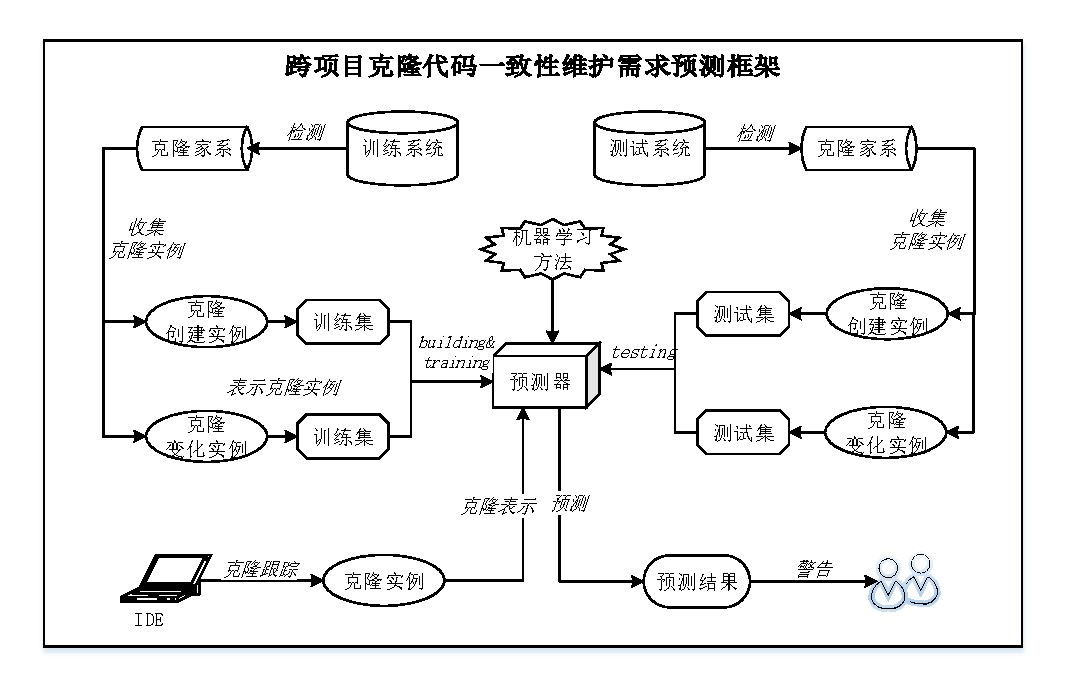
\includegraphics[width = 0.8\textwidth]{framework5.pdf}
\bicaption[framework5]{}{跨项目克隆代码一致性维护需求预测方法}
{Fig.$\!$}{The approach for clone cross-project consistency prediction}
\vspace{-1em}
\end{figure}

为了收集不同系统中的克隆代码创建和变化实例,同样通过构建系统的克隆家系来完成收集工作。使用NiCad来检测软件版本中的所有克隆,并通过在相邻版本的克隆组之间进行映射来构建克隆家系,用于收集克隆实例。然后,通过提取属性值表示克隆创建和变化实例,分别提取代码属性和上下文属性表示克隆创建实例,提取代码属性、上下文属性和历史属性表示克隆变化实例。最后,使用收集到的训练系统的克隆实例训练机器学习模型,并使用其预测测试系统的克隆代码一致性维护需求。

每一个克隆实例有两种不同的预测结果,即满足一致性维护需求和不满足维护需求。对于满足一致性维护需求实例来说,其在将来的演化中可能会引发一致性变化,程序开发人员需要采取相应的操作。例如,拒绝克隆创建实例或者检查克隆变化实例的一致性。对于不满足一致性维护需求实例来说,其在将来的演化中不会引发一致性变化,程序开发人员不需要采取相应的操作,可以放心自由的接受新创建的克隆实例和修改克隆代码。

本章在进行跨项目的克隆一致性维护需求预测时,将同时预测克隆代码创建时和变化时的跨项目一致性维护需求,将重点分析和讨论如下问题:

(1)在软件开发初期阶段,在项目自身训练数据不充分的情况下,能否使用其它系统的数据训练模型,并对该系统进行克隆一致性需求预测?

(2)在进行跨项目的克隆一致性维护需求预测时,应该预测哪一类别的克隆代码实例,是否对两种不同类别的实例都具有相一致的预测效果?

(3)在进行跨项目的克隆一致性维护需求预测时,训练数据将如何影响跨项目的预测效果?%应该如何选择跨项目预测的数据集,以达到更好的预测效果?

\BiSection{克隆代码一致性维护需求的定义}
{The Definitions for Clone Consistency-Requirement}

本文第3章和第4章分别提供了两种不同形式的克隆代码一致性变化定义,从而适应于不同时间的克隆一致性维护需求预测中。为了进一步研究跨项目的一致性预测问题,本节统一了第3章和第4章的定义,以应用于跨项目的克隆代码一致性维护需求预测中。首先,为更好的预测克隆代码的一致性维护需求,进一步提炼了克隆片段的一致性变化,如下所示:

\begin{definition}[克隆片段的一致性变化]  
\label{def-change}
克隆组内两个克隆代码片段 $CF_1$和 $CF_2$,被分别地修改为$CF'_1$和$CF'_2$。 如果对于一个接近于0阈值$\tau$,如果克隆代码$CF_1$和$CF_2$的变化满足以下条件,称此变化为一致性变化(Consistent Change) , 
\begin{equation}
\begin{split}
\begin{array}[t]{crl}
 \mathit{TextSim}(CF_i, CF'_i) < 1 & \forall i \in \{1,2\} &(1) \\
 \multicolumn{2}{c}{| ~\mathit{TextSim}(CF_1,CF'_1)  ~-~ \mathit{TextSim}(CF_2,CF'_2) ~| ~< ~ \tau}  & (2)
\end{array}
\end{split}
\end{equation}

如果克隆代码变化仅满足条件1,将其称为Type-1一致性变化(Type-1 Consistent Change);如果克隆变化同时满足条件1和条件2,将其称为Type-2一致性变化(Type-2 Consistent Change)。
\end{definition}

定义中克隆代码$ CF_1 $和$ CF_2 $的变化情况由相似性度量$ \mathit {TextSim} $进行定义,与第3章和第4章计算方式相同。该定义中的两个约束条件共同定义了克隆代码的一致性变化,约束条件$1$确保了克隆代码片段同时被修改,约束条件$2$确保克隆代码片段发生了相同的变化。

其中,Type-1一致性变化表示克隆创建时的一致性变化,Type-2一致性变化表示克隆变化时的一致性变化。这两种不同的一致性变化,将分别应用于两种不同时间的克隆一致性维护需求预测中。在克隆代码创建时,目标是避免新创建的克隆代码在其未来演化过程中的一致性变化,及其所导致额外的维护代价。所以,只要两个克隆片段同时变化,即认为会导致额外维护代价。因此,在克隆代码创建时使用Type-1的一致性变化。在克隆代码变化时,目的是避免克隆变化可能导致的未来演化中的一致性违背缺陷。所以, 不仅要求两个克隆代码片段同时变化,还需要发生相同的变化,否则将会引入克隆一致性违背缺陷,因此,在克隆代码变化时使用Type-2一致性变化。

在克隆演化过程中,克隆片段是以克隆组的形式出现在软件系统中。克隆代码的变化情况必然会导致克隆组的变化,而克隆组的变化使用一致性变化模式描述。根据克隆片段一致性变化定义,可给出克隆组的一致性变化模式定义,如下所示:

\begin{definition}[克隆一致性变化模式] 
\label{def-pattern}
在软件版本 $j+1$中存在一个克隆组$CG'$ ,假设克隆组内至少存在两个克隆代码片段$CF'_1$ 和 $CF'_2$可以与映射到上一版本$j$的克隆组$CG$中,且 $CG$中与之对应的克隆代码片段的 $(CF_1,CF_2)$被修改为$(CF'_1,CF'_2)$。如果克隆片段之间的变化 $(CF_1,CF_2)$变化至$(CF'_1,CF'_2)$满足克隆片段的“Type-1或者Type-2一致性变化”(Type-1 or Type-2 Consistent Change),则称克隆组$CG'$具有Type-1或者Type-2一致性变化模式(Type-1 or  Type-2 Consistent Change Pattern)。
\end{definition}

回顾本章地研究内容是,在两种不同的时刻预测克隆代码的一致性维护需求,结合第3章和第4章的克隆实例的定义,这里将克隆创建实例和克隆变化实例统一为克隆实例,如下所示:

\begin{definition}[克隆实例] 
\label{def-instance}
将克隆创建实例和克隆变化实例统称为克隆实例。在一个克隆家系$CG$中,克隆家系的根节点为克隆创建实例,并且发生变化的克隆组为克隆变化实例。
\end{definition}

克隆实例在演化过程中可能会发生一致性变化,从而导致额外的维护代价;同时如果不能确保克隆组的一致性,也会导致一致性违背缺陷。具体来说,对于克隆创建实例,Type-1一致性变化可能会导致额外的克隆维护代价。对于克隆变化实例,Type-2一致性变化可能会导致克隆一致性违背缺陷。因此,需要在不同时间预测克隆实例的一致性维护需求,以避免额外的克隆维护代价和一致性违背缺陷。本章结合第3章和第4章的克隆代码一致性维护需求的定义,将克隆创建和变化的一致性维护需求统一为克隆一致性维护需求定义,如下所示:

\begin{definition}[克隆一致性维护需求] 
 \label{def-requirement}
给定版本 $j$中一个克隆实例,即克隆创建实例或者克隆变化实例,如果在版本$k$中存在一个克隆组 $CG'$($k>j$)满足以下条件: (1) 在$CG'$中至少存在两个克隆片段在其克隆家系$CGE$中可以映射到克隆实例 $CG$中, (2) $CG'$ 具有“Type-1或者Type-2一致性变化模式”(Type-1 or Type-2 Consistent Change Pattern),则称克隆实例$CG$满足克隆一致性维护需求(Consistency-Requirement);反之,如果不存在克隆实例,称该克隆实例$CG$不需要一致性维护(Consistency-Requirement Free,或者Consistency-Free,或者Free)。
其中,克隆创建实例和克隆变化实例的一致性维护需求分别满足Type-1和Type-2一致性变化模式。
\end{definition}

最终,克隆一致性维护需求预测可以转化为以下问题:给定一个克隆实例(即克隆创建实例或者克隆变化实例),判断该克隆实例是否满足克隆一致性维护需求。

\BiSection{跨项目数据集的获取}
{Collecting the Dataset for Cross-Project Prediction}

在跨项目的预测中,使用其它系统的数据训练机器学习模型,并预测另外系统的一致性维护需求。因此,需要构建跨项目的数据集,将从训练系统中提取克隆实例作为训练集,从测试系统中提取克隆实例作为测试集。对于某一个软件系统来讲,通过收集和表示该系统中的克隆实例,可以生成其数据集。因此,生成实验所需的数据集,可以划分为两个部分:收集系统中的克隆实例和表示所收集到的克隆实例。

\BiSubsection{跨项目数据来源}
{Data Sources for Cross-Project Prediction}

跨项目的数据由软件系统中的克隆实例组成,因此收集系统中的克隆实例,即可以完成收集跨项目的数据。通过构建系统的克隆家系,通过识别其中的克隆演化模式,可以从软件中收集所有的克隆实例。根据定义~\ref{def-instance}~,克隆家系$CGE$中的初始节点即是克隆创建实例,发生变化的克隆组是变化实例。通过构建和遍历克隆家系,可以收集克隆创建和变化实例。所采用的方法与本文第3章和第4章的方法类似,但在跨项目预测中,需要同时收集克隆创建和克隆变化实例。

首先,下载系统所有版本的源代码,通过映射所有相邻版本的克隆代码,构建系统中全部克隆家系。然后,通过对比相邻版本的克隆代码,识别克隆家系的克隆演化模式,尤其是克隆一致性变化模式(参考定义~\ref{def-evolutionpattern}~和\ref{def-pattern}~)。根据定义~\ref{def-instance}~通过遍历克隆家系的根节点,可收集系统中所有的克隆创建实例。在收集克隆创建实例后,还需确认该实例中的被复制和被粘贴代码(参见本文第3章收集克隆创建实例小节~\ref{lab-checkcopied}~)。根据定义~\ref{def-instance}通过识别克隆家系中的变化克隆组,便可以收集系统中的克隆变化实例。

根据定义~\ref{def-requirement}~,通过遍历克隆实例所在的克隆家系$CGE$的演化情况,标识克隆实例的一致性维护需求。如果克隆实例在其演化过程中发生了一致性变化模式(定义~\ref{def-pattern}~),则该实例满足一致性维护需求,否则不满足维护需求。

\BiSubsection{数据集生成}
{Generating All the Data Set}

本文收集到的数据是系统中的克隆实例,因此同样提取相应的属性值表示克隆代码实例。将提取代码、上下文两组属性代表克隆创建实例,提取代码属性、上下文属性和演化属性代表克隆变化实例。其中,代码属性和上下文属性相似,但从不同的角度表示克隆创建实例和变化实例。克隆创建实例中的属性,表示了创建时克隆代码的特征;克隆变化实例中的属性,表示了发生变化的克隆组的特征。

数据集生成算法如~\ref{alg-collection}~所示。算法中第1行是使用第2章的克隆家系构建算法生成克隆家系并识别克隆演化模式。第2 - 4行是根据第3和4章的算法收集克隆创建和变化实例,并标记其一致性维护需求。第5行是初始化数据集。第6 - 8行是提取相应的属性值表示克隆实例,并且生成数据集。在表示克隆实例时,算法将消耗大量的时间,其时间复杂度为$O(m*n)$,其中$m$为克隆变化实例的数量。因此,该算法的时间复杂度为$O(m*n)$。

\vspace{1em}
\begin{minipage}{0.8\textwidth}
\centering
\begin{algorithm}[H]
\AlgoBiCaption{数据集生成算法} {The algorithm for generating dataset}
\label{alg-collection}
\KwIn{All source code and code clones from $N$ versions}
\KwOut{The data set of software}
Generating all clone genealogies $CGEs$ with number $N\_cge$ according to~Algo.~\ref{alg-building}~\;
\For{$i$=1 to $N\_cge$}
{ 
 Collecting the clone instance that both including clone-creating and changing instances from $CGE\_i$ according to Algo.~\ref{alg-collectioncreating}~and~Algo.~\ref{alg-collectionchanging}~\; 
 Labeling all consistency-requirement according to Definition~\ref{def-requirement}~;
}
Initializing all training data set $Creating\_Set$ and $Changing\_Set$ for clone creating and changing instances\; 
\For{each clone instance} 
{ 
Generating all attributes for clone creating or changing instance according to Algo.~\ref{alg-creatingperdition}~and~Algo.~\ref{alg-changingperdition}~\;
Appending all the attributes to the $Creating\_Set$\ or $Changing\_Set$\;
}
\Return {The data set of software\;}
\end{algorithm}
\end{minipage}
\vspace{1em}

对于克隆创建实例,提取与第3章相同的属性特征,具体信息可以参考本文第~\ref{lab-creatingattribute}~节克隆创建实例表示。使用代码属性用于表示被复制的克隆代码的特征,包括:克隆代码粒度、Halstead属性、结构属性、参数访问数量、总函数调用次数、本地函数调用次数、库函数调用次数、其它调用次数。使用上下文属性用于表示被粘贴的克隆代码的特征,包括:代码相似度、局部克隆标识、文件名相似度、文件名相似度标识、方法名相似度、总参数名相似度、最大参数名相似度、总参数类型相似度、块信息标识。

对于克隆变化实例,提取与第4章相同的属性特征,具体信息可以参考本文第~\ref{lab-changingattribute}~节克隆变化实例表示。从克隆组的角度重新提取了代码属性和上下文属性,并从演化的角度新增演化属性。代码属性从代码自身的角度,描述了克隆变化实例中克隆代码特征,包括克隆粒度、代码行平均、Halstead属性平均、结构属性平均、总函数调用次数平均、本地函数调用次数平均、库函数调用次数平均、其它调用次数平均。上下文属性描述了克隆变化实例所在克隆组的克隆关系特征,包括代码相似度平均、文件名相似度平均、文件名相似度变量、方法名相似度平均、总参数名相似度平均、最大参数名相似度平均、总参数类型相似度平均、块信息标识。历史属性描述了克隆变化实例所在克隆组在克隆变化发生前的历史演化特征,包括变化实例寿命、历史演化模式统计、当前演化模式、历史变化统计。同时,还提供了克隆变化实例的变化属性。

%%%\begin{minipage}{0.8\textwidth}
%%%\centering
%%%\begin{algorithm}[H]
%%%\AlgoBiCaption{数据集生成算法} {The algorithm for generating dataset}
%%%\label{alg-collection}
%%%\KwIn{All source code and code clones from $N$ versions}
%%%\KwOut{The data set of software}
%%%\For{$i$=1 to $N$}
%%%{ 
%%% Generating CRD to represent each code clone{CFs}\;
%%% Mapping all the $CFs$ and $CGs$ between the adjacent versions {i} and {i+1}\;
%%% Identifying all clone evolution pattern in thus two versions according to Definition~\ref{def-evolutionpattern}~and~Definition~\ref{def-pattern}~\;
%%%}
%%%Generating all clone genealogies $CGEs$ with number $N\_cge$\;
%%%\For{$i$=1 to $N\_cge$}
%%%{ 
%%% Collecting the clone instance that both including clone-creating and changing instances from $CGE\_i$ according to Definition~\ref{def-instance}~\; 
%%% Labeling all consistency-requirement according to Definition~\ref{def-requirement}~;
%%%}
%%%Initializing all training data set $Creating\_Set$ and $Changing\_Set$for clone creating and changing instances\; 
%%%\For{each clone instance} 
%%%{ 
%%%Generating all attributes for clone creating or changing instance\;
%%%Appending all the attributes to the $Creating\_Set$\ or $Changing\_Set$\;
%%%}
%%%\Return {The data set of software\;}
%%%\end{algorithm}
%%%\end{minipage}

%%%%数据集生成算法如~\ref{alg-collection}~所示。算法中第1-5行是为克隆代码生成CRD,并使用CRD映射相邻版本的克隆代码,并根据克隆演化模式定义,识别克隆演化模式。第6行是生成系统的克隆家系。第7-10行,分别是收集克隆实例,并标记其一致性维护需求。第11行是初始化数据集。第12-15行是提取相应的属性值表示克隆实例,并且生成数据集。在表示克隆实例时,算法将消耗大量的时间,其时间复杂度为$O(m*n)$,其中m为克隆变化实例的数量。因此,该算法的时间复杂度为$O(m*n)$。

\BiSection{跨项目预测模型的训练与预测}
{Training the Cross-Project Models and Predicting}

使用收集到的训练系统的克隆实例训练机器学习模型,并预测测试系统的克隆代码的一致性维护需求。从而验证跨项目的克隆一致性需求的预测能力。值得注意的是,将对两种不同的时刻的克隆代码的一致性维护需求分别进行预测(即克隆创建时和克隆变化时),因此会训练两种不同的模型以适用于两个时刻。

对于所测试的软件系统,首先,通过收集训练系统中所有的克隆实例(创建实例和变化实例),并提取相应的属性,用于构建模型训练所需的数据集。然后,调用WEKA中的机器学习算法,分别构建克隆创建和变化的预测器,预测克隆代码的一致性维护需求。

与第3章和第4章相似,根据定义~\ref{def-requirement}~,克隆实例会有两种不同的状态:需要一致性维护和不需要一致性维护。如下所示:

\begin{itemize}
\item 
需要一致性维护:
若克隆创建实例的预测结果为“需要”,软件开发人员需要谨慎的执行克隆创建操作。因为,该克隆创建实例,在未来演化的过程中可能会引发一致性变化,从而向系统中引入额外的维护代价。若克隆变化实例的预测结果为“需要”,软件开发人员需要检测克隆变化实例所在的克隆组的一致性问题,考虑一致地修改组内其它的克隆代码。因为该克隆变化实例,在未来演化的过程中可能会引发一致性变化,遗忘这种变化会向系统中引入缺陷,从而降低软件质量。
\item
不需要一致性维护:
若克隆创建实例的预测结果为“不需要”,软件开发人员可以自由的执行克隆创建操作,从而节约开发时间提高开发效率。因为该克隆创建实例,在未来演化的过程中不会引发一致性变化,也不会导致额外的维护代价。若克隆创建实例的预测结果为“不需要”,软件开发人员可以自由的修改克隆变化实例所在克隆组的克隆片段。因为,该克隆变化实例,在未来演化的过程中不会引发一致性变化,也不会导致一致性违背缺陷。
\end{itemize}

跨项目克隆一致性维护需求预测算法如~\ref{alg-crossperdiction}~所示。算法的第1行为划分训练集和测试集。第2 - 3行是生成跨项目的数据集。第4行是使用训练集训练机器学习模型。第5行是使用训练的模型在测试集上验证跨项目预测的有效性。

\vspace{1em}
\begin{minipage}{0.8\textwidth}
\centering
\begin{algorithm}[H]
\AlgoBiCaption{跨项目克隆一致性维护需求预测算法} {The algorithm for cross-project predicting clone consistency}
\label{alg-crossperdiction}
\KwIn{All the projects}
\KwOut{The predictive models}
Dividing the projects into training projects and testing project\;
Generating the $Training\_{Set}$ for training projects\;
Generating the $Testing\_{Set}$ for testing project\;
Calling WEKA to train the models applying training set $Training\_{Set}$\;
Employed this trained model to predict on the $Testing\_{Set}$\;
\Return {The predictive models\;}
\end{algorithm}
\end{minipage}
\vspace{1em}

在使用已训练好的模型进行预测时,可以与软件开发过程相结合,将该模型嵌入到软件开发环境中,帮助程序开发人员实现边开发边预测克隆实例的一致性维护需求。首先,在软件开发环境中需监测和跟踪克隆代码,识别新产生的克隆实例(克隆创建实例和变化实例)。然后,根据上文描述的代码、上下文和演化属性,提取相应的特征表示相应的克隆实例。最后,使用训练好的预测器预测相应克隆实例的一致性维护需求,根据预测结果提醒程序开发人员采取进一步的操作。

\BiSection{克隆一致性维护需求预测插件的设计与实现}
{Design and Implementation for the Plug-in of Clone Consistency-Requirement Prediction}

为了与软件开发过程相结合,在软件开发过程中对克隆代码进行一致性维护需求预测,本文还设计并实现了一个克隆代码的一致性维护需求插件。

本文所设计的插件是基于eclipse的插件环境实现的,因此可以嵌入到软件开发环境中(eclipse),帮助软件开发人员实现边开发、边预测、边维护克隆代码的一致性维护需求。在软件开发过程中,基于eclipse的预测插件可以帮助程序开发人员避免克隆变化导致的一致性维护代价及一致性违背缺陷,从而提高软件质量和可维护性。

\BiSubsection{克隆一致性维护需求预测插件的体系结构}
{The Architecture for the Plug-in of Clone Consistency Prediction}

本文所设计的克隆代码一致性维护需求预测插件的体系结构如图~\ref{pluginarchitecture}~所示,从上到下依次分为交互层、控制层、功能层、传输层、数据层。

\begin{figure}[h]
\centering
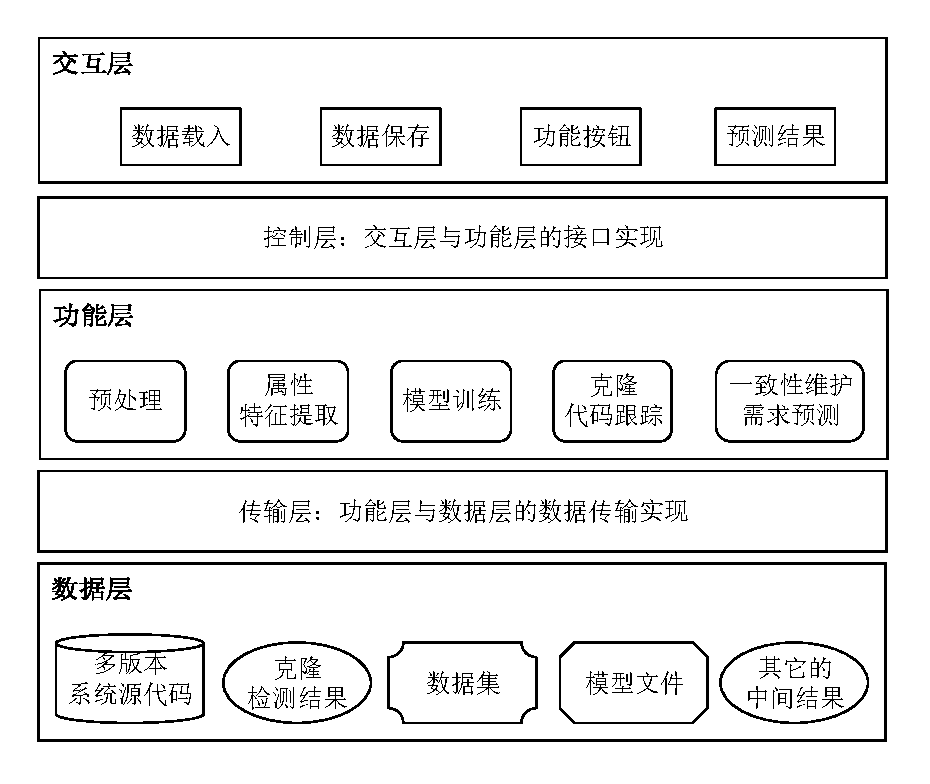
\includegraphics[width = 0.7\textwidth]{pluginarchitecture.pdf}
\bicaption[pluginarchitecture]{}{克隆一致性维护需求预测插件的体系结构}{Fig.$\!$}
{The architecture for the plug-in of clone consistency-requirement prediction}
\vspace{-1em}
\end{figure}

交互层是面向开发人员的展示层,开发人员可以通过该层与插件进行交互。通过“数据载入”可以载入相应的数据,并在操作界面中选择不同的“功能按钮”来调用插件相应的功能,还可以将一些中间数据进行保存。同时,交互层还可以向开发人员提供克隆一致性维护需求预测的结果,通知开发人员采取相应的操作。

控制层主要负责交互层与功能层之间的接口实现。通过控制层对开发人员的交互层请求进行响应,并然后调用功能层完成特定的功能。当完成特定功能后,控制层还会将功能层所返回的结果反馈给交互层。

功能层是本文插件的的核心所在,实现了克隆代码一致性维护需求预测的核心功能,在整个插件中起到了最关键的作用。功能层实现了五个不同的功能模块,包括预处理模块、属性特征提取模块、模型训练模块、克隆代码跟踪模块和一致性维护需求预测模块。功能层通过接受用户所指定的输入数据,并实现相应的功能完成用户的需求。

传输层负责数据层与功能层之间的数据交换与传输。在考虑代码的一致性维护需求预测中,需要一些输入数据的支持,比如系统源代码和克隆检测工具。传输层所负责的即是数据的传输。

插件的最后一层是数据层,可以向插件提供基本的数据以及一些必要的输出等。在本文设计的插件中,数据层数据主要包括系统源代码数据、克隆代码检测结果数据、功能层生成的机器学习训练集数据、模型文件以及其它的一些中间结果等。

\BiSubsection{克隆一致性维护需求预测插件的功能模块设计}
{The Design for Plug-in Function Modules of Clone Consistency Prediction}

本文的克隆代码一致性维护需求预测插件主要包括五个模块:预处理模块、属性提取模块、模型训练模块、克隆跟踪模块和预测模块。插件的模块设计如图~\ref{pluginmodule}~所示。预处理模块构建克隆家系并识别克隆演化模式,帮助程序开发人员收集系统中的克隆实例。属性提取模块实现对克隆实例的表示,提取不同的属性组表示相对应的克隆实例。预测模块可以根据不同用户需求,通过调用WEKA中的机器学习算法,构建和训练克隆一致性维护需求的预测器。克隆跟踪模块可以跟踪系统中的克隆代码产生和变化。预测模块可以根据克隆跟踪的过程,对新产生的克隆代码和克隆代码的变化进行一致性维护需求预测。

\begin{figure}[h]
\centering
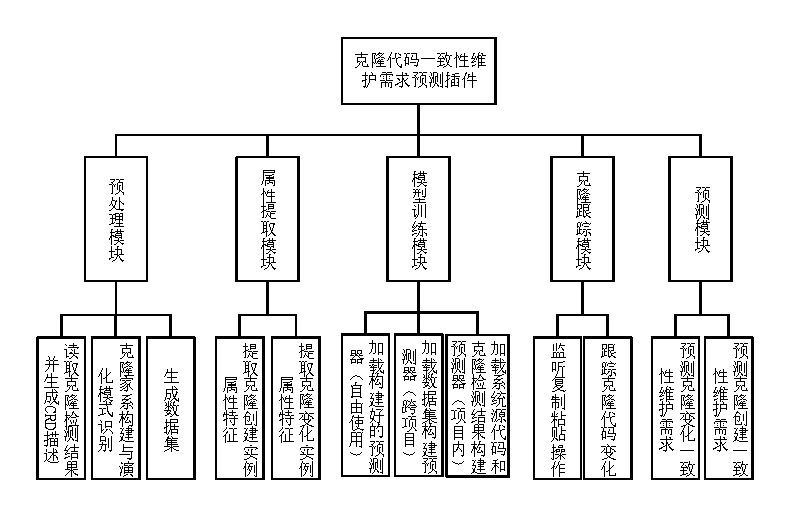
\includegraphics[width = 0.8\textwidth]{pluginmodule.pdf}
\bicaption[pluginmodule]{}{克隆一致性维护插件的功能模块}{Fig.$\!$}
{The modules for clone consistency-requirement prediction}
\vspace{-1em}
\end{figure}

(1)预处理模块

预处理模块通过识别克隆检测工具的检测结果,并构建克隆家系和识别克隆演化模式,从而收集并生成相应系统的克隆实例。首先,需要人工的使用克隆检测工具检测系统中的所有的克隆代码,并将检测结果作为插件的输入,本文中使用的克隆检测工具是NiCad 。对于软件系统的每一个版本,克隆代码将会被组成克隆组的形式,并使用文件名、起始行号表示所有的克隆代码,即“{file\_name}”、“{start\_line}”和“{end\_line}”。然后,使用CRD重新描述克隆代码并重新组织为新的数据结构,从而方便构建克隆家系。然后,本插件将基于CRD对所有版本中的克隆代码,构建构建系统的克隆家系,并识别克隆演化模式。方法见本文克隆家系构建和模式识别部分。最后,根据所构建的克隆家系和识别的演化模式,可以方便的生成相应系统的克隆创建和变化实例,从而生成其相应的数据集。值得注意的是,完整的数据集需通过调用属性提取模块生成具体的属性特征。

(2) 属性提取模块

属性提取模块可以提取克隆实例的属性特征,将不同的克隆代码实例抽象成相应的属性值。对克隆创建实例,提取代码属性表示被复制的克隆代码,提取上下文属性表示被粘贴的克隆代码。对克隆变化实例,从克隆组的角度提取代码属性、上下文属性、演化属性和相对应的克隆变化情况。首先,对代码属性和上下文属性的提取,可以使用抽象语法树(Abstract Syntactic Tree,AST)对程序源代码进行解析并提取。对每一个克隆代码以及克隆代码所在文件,使用Eclipse AST中的 ASTParser类将克隆片段所在源代码解析成AST\footnote{抽象语法树可参见:http://www.eclipse.org/articles/Article-JavaCodeManipulation\_AST/}。通过遍历语法树访问相应关键节点,根据本文描述的属性值计算克隆实例的代码属性和上下文属性。然后,对于演化属性的提取,可以取通过遍历该克隆实例的克隆家系,根据对其属性的描述计算相应演化属性。

(3)模型训练模块

模型训练模块根据用户的请求,调用WEKA构建和训练机器学习模型。为灵活的使用本文方法,本文提供三种构建和训练预测模型的方式:

(a)项目内模型训练,该方式用项目自身的历史数据来训练预测模型。在这种情况下,本文的插件首先调用预处理模块,构建项目本身所有克隆家系和收集项目中的所有克隆实例。然后调用属性提取模块,将提取收集到的克隆实例的属性值,并生成训练集。最后,使用该训练集建立和训练机器学习模型,并将训练好的模型应用于克隆代码的一致性维护需求预测中。

(b)跨项目模型训练,该方式使用其它项目数据作为训练集来训练预测模型。在软件开发初期,由于演化时间较短导致其历史的克隆实例较少,不足以较好的训练所需要的模型。因此,需要使用其它项目的历史数据作为训练集。首先,用户指定相应的训练系统,并导入相应的输入数据。然后,通过调用预处理和属性特征提取模块生成所需的训练集。最后,使用训练集训练跨项目的预测模型,并将其应用于当前测试系统的一致性维护需求预测中。需要注意的是,随着时间的推移,当项目自身可以收集到足够的数据时,本文建议开发人员重新使用项目自身的数据训练机器学习模型,从而达到较好的预测效果。

(c)加载已有训练模型,该方式直接加载已经训练好的机器学习模型。由于机器学习模型的构建和训练往往需要大量的时间,开发人员不应该也不需要在每次开发时都训练机器学习模型。因此,在实际的开发过程中,模型的训练和开发时的预测可以分开进行。首先通过(a)和(b)两种方式进行模型的训练,然后使用(c)加载训练好的模型文件,最后进行克隆代码一致性维护需求预测。

(4)克隆代码跟踪模块

在软件开发过程中预测克隆代码的一致性需求维护,还需要实时的捕获软件中产生的克隆实例,即跟踪克隆实例的产生(克隆创建实例和克隆变化实例)。

首先,该模块可以跟踪开发人员的复制和粘贴操作。研究表明,软件中的克隆代码主要是由于复制和粘贴操作导致,即克隆创建实例产生的直接原因是程序开发人员的复制和粘贴操作。因此,监测复制和粘贴操作即可跟踪克隆创建实例的产生。但是,在实际的软件开发过程中,大部分的复制和粘贴操作是对一些具体的变量进行的,这些操作不会导致克隆代码。因此,本文对复制粘贴操作进行了筛选,认定复制和粘贴的代码行数最少为5行的操作,才是会导致克隆代码的复制和粘贴操作。

然后,该模块还可以跟踪系统中克隆代码的变化。对克隆代码跟踪的功能有两种实现的策略,一是根据CRD跟踪演化的克隆代码,而是通过eclipse开发平台所提供的文档内片段位置更新功能(位置更新器)实现。对于第一种方式,克隆代码的CRD中存储了其上下文信息,通过比较开发人员当前修改的代码片段是否和系统中的克隆代码区域重合,认定是否对克隆代码片段进行了修改。对于第二种方式,对于一个打开的文档,先确定该文档内是否含有克隆代码,如果含有克隆代码,则需要对其包含的克隆代码进行跟踪。位置跟踪器通过克隆代码片段的首字符在文档中的偏移量和片段长度来表示要跟踪的范围。将要跟踪的代码片段位置和跟踪其位置的更新器通过更新器种类绑定在一起,便可实现克隆片段的位置跟踪。然后,通过判断该克隆代码片段是否被修改(与上一版本比较),识别克隆代码的变化。

(5)预测模块

当监测到具体的克隆实例产生时,调用已经训练好的机器学习模型进行预测。软件开发过程中,监测到克隆实例产生时,调用属性提取模块提取本次实例的属性,并使用训练好的一致性模型预测其一致性维护需求。根据预测结果通知程序开发人员采取相应措施。值得注意的是,在实际预测时,克隆变化实例预测需要项目的历史版本源代码,因为历史属性中包含克隆变化实例的历史变化过程。为了轻量化预测过程,程序开发人员可以将当前版本中所有的克隆组的演化属性均提取出来。当克隆变化实例产生时,直接使用其作为属性,从而降低属性提取的时间。

%%%\BiSubsection{克隆一致性维护需求预测插件的总体框架}
%%%{The Framework for Plug-in of Clone Consistency Prediction}
%%%
%%%本文的克隆代码一致性维护需求预测插件的系统整体框架如图\ref{pluginframework}所示。

%%\begin{figure}[h]
%%\centering
%%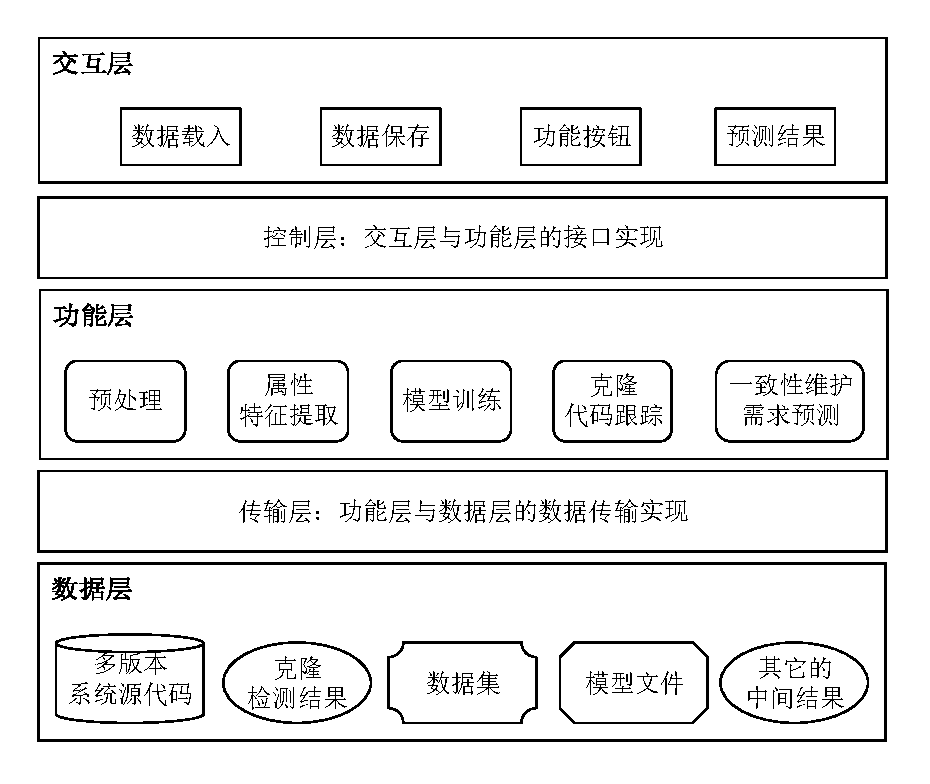
\includegraphics[width = 0.7\textwidth]{pluginframework.pdf}
%%\bicaption[pluginframework]{}{克隆一致性维护需求预测插件的体系结构}{Fig.$\!$}
%%{The framework for the plug-in of clone consistency-requirement prediction}
%%\vspace{-1em}
%%\end{figure}

\BiSubsection{克隆一致性维护需求预测插件的实现}
{The Implementation for Plug-in of Clone Consistency Prediction}

本文基于eclipse实现了克隆一致性维护需求预测插件。eclipse 是一个基于Java语言的开源集成开发环境,具有良好的可扩展性和跨平台性。eclipse是一个具有极小内核的开发平台,其所有功能都以插件的形式添加到此内核上。同时,eclipse具有极为友好的插件开发环境,用户可以根据自身需要开发所需的功能,并以插件的形式发布在eclipse平台上。因此,本文也选择ecilpse实现克隆代码的一致性维护需求预测插件。

同时,本文设计的插件需要对不同的机器学习模型进行训练,并对在软件开发过程进行一致性维护需求预测。为了实现此功能,本插件也集成了WEKA的软件开发包。WEKA是一个Java语言实现的数据挖掘和机器学习开源工具,提供了丰富的接口帮助程序开发人员调用相关的机器学习方法,从而极为灵活的进行模型的训练和预测\footnote{使用WEKA可参见:http://weka.wikispaces.com/。}。

本文所设计的插件运行截图如图~\ref{pluginview1}~所示。由图中看出,本章实现的插件会在eclipse开发环境的菜单栏中,新增加一个新的菜单项“Clones”。该菜单具备克隆一致性维护需求预测的功能\footnote{本文所设计的插件见:https://github.com/zhangfanlong/CloneControlPlug-in。欢迎开发人员在实际开发过程中使用本文的所提出的克隆代码一致性维护需求预测方法,并期望给出建议与意见。}。

\begin{figure}[htbp]
\centering
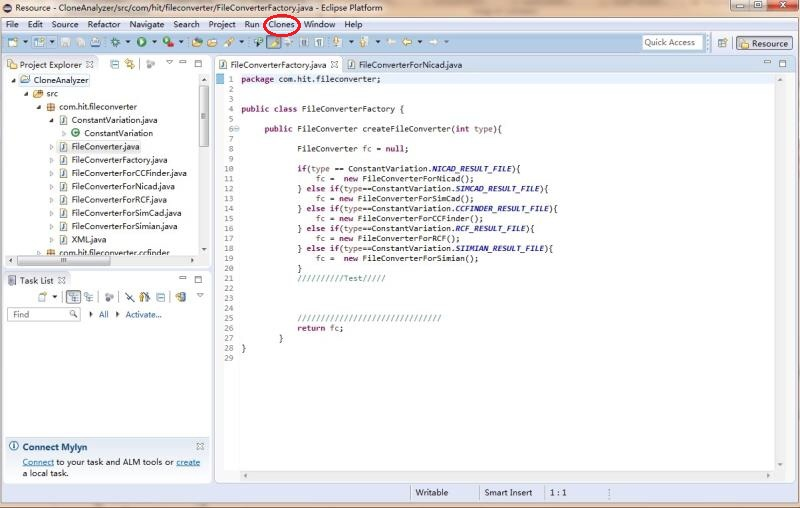
\includegraphics[width = 0.8\textwidth]{plugin1.jpg}
\bicaption[pluginview1]{}{插件安装完成后eclipse界面}{Fig.$\!$}
{The screen-shot for eclipse with installed plug-in of clone consistency prediction}
\vspace{-1em}
\end{figure}

在使用本文所设计的一致性维护需求预测插件时,需要提前加载已训练好的机器学习模型。为方便用户使用,本章插件提供三种方式加载预测模型:(1)加载系统源代码及克隆检测工具的检测结果构建预测模型(项目内);(2)加载已有软件历史版本特征向量训练预测模型(跨项目)。(3)加载已有预测模型。加载所需功能截图如图~\ref{pluginview2}~所示。

\begin{figure}[htbp]
\centering
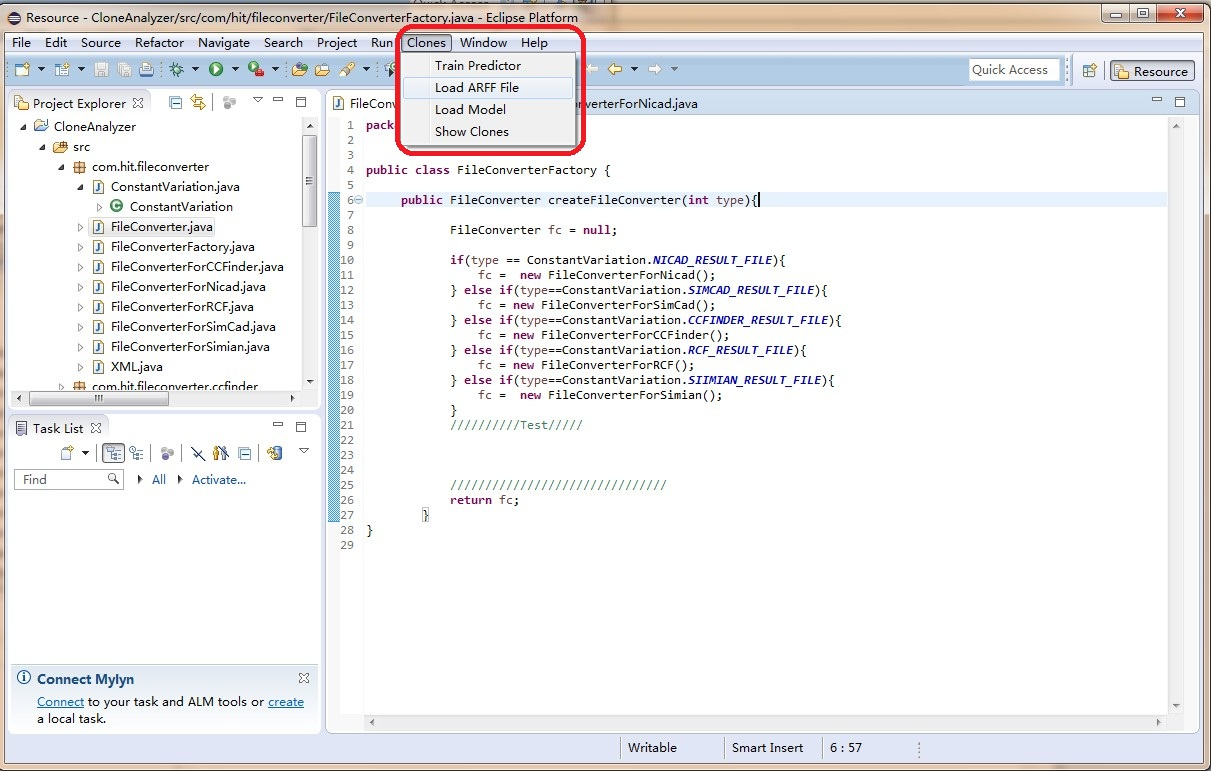
\includegraphics[width = 0.8\textwidth]{plugin2.jpg}
\bicaption[pluginview2]{}{插件加载预测模型的截图}{Fig.$\!$}
{The screen-shot for loading the models of clone consistency prediction}
\vspace{-1em}
\end{figure}

成功加载预测模型后,该插件便可以预测克隆代码的一致性维护需求。通过监听开发过程中的克隆创建和变化实例,并预测克隆代码的一致性维护需求。图中~\ref{pluginview3}~是一个会导致额外维护代价的克隆创建操作的警告示例。如图所示,本插件会警告软件开发人员,其操作会引发额外的维护代价。根据预测结果,开发人员可以采取拒绝此复制粘贴操作,以避免在其未来演化过程中的克隆代码的额外维护代价。

\begin{figure}[htbp]
\centering
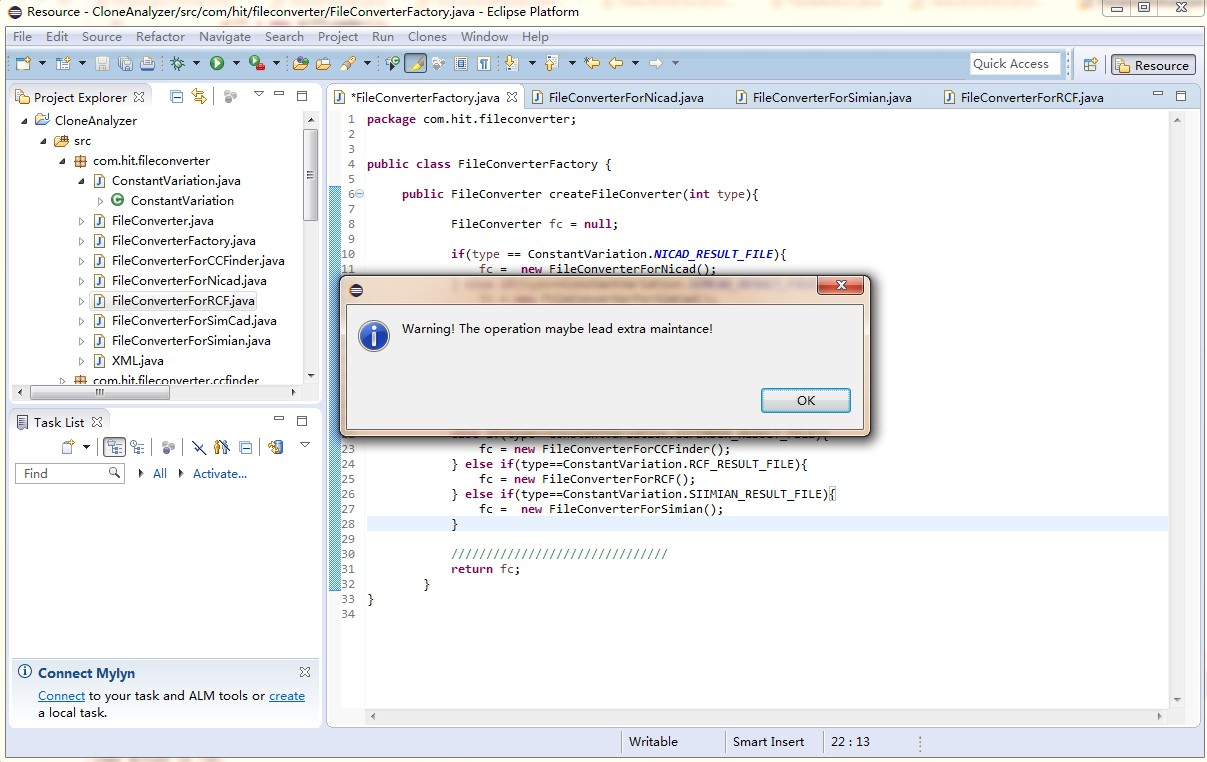
\includegraphics[width = 0.8\textwidth]{plugin3.jpg}
\bicaption[pluginview3]{}{需要一致性维护的预测结果示例}{Fig.$\!$}
{The screen-shot for a prediction example that meeting consistency}
\vspace{-1em}
\end{figure}

\BiSection{实验结果与分析}
{Experimental Results and Analysis}

\BiSubsection{实验设置}
{Experimental Methodology}

本章在四个Java开源系统上进行实验评估,所收集的克隆实例的统计信息如表~\ref{instancesta}~所示。从该表可以看出,系统中克隆创建实例的数据集的规模要大于克隆变化实例的数据集。克隆创建实例数据集规模为633到3666个,克隆变化实例的数量范围在159到1040个。

\begin{table}[h]
\bicaption[instancesta]{}{跨项目的测试集信息统计}
{Table$\!$}{The statistics for cross-project testing data}
\vspace{0.5em}
\centering
\wuhao
\begin{tabular}{ccccc}
\toprule[1.5pt]
~\multirow{2}{*}{类型}&\multirow{2}{*}{测试系统}&\multicolumn{3}{c}{测试集规模}\\
\cline{3-5}
~&~&{不需要维护}&{需要维护}&{总数}~\\
\midrule[1pt]
\multirow{4}{*}{克隆创建实例}
&ArgoUML&	2574(77.07\%)&	766(22.93\%)&	3340\\
&jEdit&560(88.47\%)&	73(11.53\%)&	633\\
&jFreeChart&	2013(59.80\%)&	1353(40.20\%)&	3366\\
&Tuxguitar&	1016(71.10\%)&	413(28.90\%)&	1429\\
\hline
\multirow{4}{*}{克隆变化实例}
&ArgoUML&288(67.45\%)&139(32.55\%)&427\\
&jEdit&78(49.06\%)&81(50.94\%)&159\\
&jFreeChart&452(43.46\%)&588(56.54\%)&1040\\
&Tuxguitar&91(25.71\%)&263(74.29\%)&354\\
\bottomrule[1.5pt]
\end{tabular}
\end{table}

在进行跨项目的预测实验时,使用三个系统的数据作为训练集,使用第四个系统作为测试集。跨项目预测的训练集如表~\ref{crosssta}~所示。表中使用(To Project)表示被测试的系统为“Project”,并使用除“Project”系统外其它的系统作为训练集。从表中发现克隆创建的训练集规模要远远大于克隆变化的训练集规模,其中克隆创建的训练集规模为5402 - 8135,克隆变化的训练集规模为940 - 1821。

\begin{table}[h]
\bicaption[crosssta]{}{跨项目的训练集信息统计}
{Table$\!$}{The statistics for cross-project training data}
\vspace{0.5em}
\centering
\wuhao
\begin{tabular}{ccccc}
\toprule[1.5pt]
~\multirow{2}{*}{类型}&\multirow{2}{*}{训练系统}&\multicolumn{3}{c}{训练集规模}\\
\cline{3-5}
~&~&{不需要维护}&{需要维护}&{总数}~\\
\midrule[1pt]
\multirow{4}{*}{克隆创建实例}
&(To ArgoUML)&3589(66.12\%)&1839(33.88\%)&5428\\
&(To jEdit)&5603(68.88\%)&2532(31.12\%)&8135\\
&(To jFreeChart)&4150(76.82\%)&1252(23.18\%)&5402\\
&(To Tuxguitar)&	5147(70.13\%)&2192(29.87\%)&	7339\\
\hline
\multirow{4}{*}{克隆变化实例}
&(To ArgoUML)&621(39.99\%)&932(60.01\%)&1553\\
&(To jEdit)&831(45.63\%)&990(54.37\%)&1821\\
&(To jFreeChart)&457(48.62\%)&483(51.38\%)&940\\
&(To Tuxguitar)&	818(50.31\%)&808(49.69\%)&1626\\
\bottomrule[1.5pt]
\end{tabular}
\end{table}

为解决跨项目克隆代码一致性维护需求预测问题,本章将研究问题划分为三个子研究问题。因此本节也从三个不同的角度进行实验评估,并回答所提出的三个子研究问题:
\begin{itemize}
\item
跨项目有效性验证实验:将回答第一个子研究问题,使用不同的机器学习模型进行跨项目克隆一致性预测,以验证是否能使用跨项目的数据进行跨项目一致性维护需求预测。
\item
跨项目使用模式实验:将回答第二个子研究问题,将探讨在进行跨项目预测时,不同类别克隆实例的一致性预测的效果。实验将使用贝叶斯网络预测不同类别的克隆实例。
\item
跨项目数据集规模实验:将回答第三个子研究问题,使用不同的数据集训练机器学习模型,并在同一系统上测试跨项目预测模型的预测能力,从而探讨训练集规模对跨项目模型预测能力的影响。
\end{itemize}

\BiSubsection{跨项目有效性验证实验}
{The Effectiveness Experiments for Cross-Project Prediction}

本节将回答本章提出的第一个研究问题:在软件开发初期阶段,在项目自身训练数据不充分的情况下,能否使用其它系统的数据训练模型,并对该系统进行克隆一致性维护需求预测?

在五种机器学习方法上进行了跨项目的预测,并使用同本文第3章和第4章相同的指标评估预测效果,即采用平均精确率(Average Precision)、平均召回率(Average Recall)和平均F值(Average F-measure)进行评价(见本文第~\ref{ref-creatingmetrics}~节和第~\ref{ref-changingmetrics}~节)。

\BiSubsubsection{克隆创建实例的实验结果}
{The Results for Clone Creating Instances}

对克隆代码创建实例,使用不同的机器学习方法进行跨项目预测,实验结果如~\ref{creatingcrossmethodaverage}~所示。表中支持向量机方法(SVM)的预测结果使用{*}进行标记表。原因在于:在跨项目克隆创建实例的一致性维护需求预测中,支持向量机方法不具备相对应的预测能力,会将所有的克隆创建实例划分到一个类别中(数量规模较大的类中)。

\begin{table}[h]
\bicaption[creatingcrossmethodaverage]{}{克隆创建实例的跨项目预测效果}
{Table$\!$}{The effectiveness of cross-project prediction for clone creating instances}
\vspace{0.5em}
\centering
\wuhao
\begin{tabular}{cccccc}
\toprule[1.5pt]
{指标}&{方法}&{To ArgoUML}&{To jEdit}&{To jFreechart}&{To  Tuxguitar}\\
\midrule[1pt]
\multirow{5}{*}{平均Precision(\%)}
&BN&	63.8	&81.2	&57.5	&64.8\\
&NB&	63.1&	78.3&	48.6&	61.5\\
%&SVM&	59.4&	78.3&	35.8&	50.6\\
&SVM&	59.4*&	78.3*&	35.8*&	50.6*\\
&KNN&	62.9&	78.6&	64.8&	58.1\\
&DT&	62.9&	79.6&	56.6&	70.4\\
\hline
\multirow{5}{*}{平均Recall(\%)}				
&BN&	67.5&	84.4&	60.2&	69.8\\
&NB&	69.3&	74.7&	54&	64.7\\
%&SVM&	77.1&	88.5&	59.8&	71.1\\
&SVM&	77.1*&	88.5*&	59.8*&	71.1*\\
&KNN&	68.7	&74.1&	64.9&	66.3\\
&DT&	74&	84.4&	59.9&	73.1\\
\hline
\multirow{5}{*}{平均F-measure(\%)}			
&BN&	65.4&	82.6&	50.8&	65\\
&NB&	65.6&	76.4&	48.9&	62.7\\
%&SVM&	67.1&	83.1&	44.8&	59.1\\
&SVM&	67.1*&	83.1*&	44.8*&	59.1*\\
&KNN&	65.3&	76.2&	60.9&	60.3\\
&DT&	66.7&	81.8&	50.3&	68.3\\
\bottomrule[1.5pt]
\end{tabular}
\end{table}

从表\ref{creatingcrossmethodaverage}~中可以看出,除了支持向量机外,其它四种机器学习方法对四个不同的系统均具有不错的预测效果。对jEdit系统的预测效果最好,平均F值在76.2\% - 82.6\%之间。同时ArgoUML系统和Tuxguitar系统的预测结果也不错,平均F值分别介于65.3\% - 66.7\%和60.3\% - 68.3\%之间。jFreeChart最差,也达到了48.9\% - 60.9\%。

尽管不同机器学习方法的预测效果不存在显著的差异,但不同的机器学习方法对不同系统具有不同的预测能力。对系统ArgoUML和系统Tuxguitar来说,决策树具有最好的预测效果,其F值分别为66.7\%和68.3\%。贝叶斯网络对jEdit系统具有最好的预测效果,F值为82.6\%。而K近邻方法对于系统jFreeChart具有最好的预测效果,F值为60.9\%。

因此,本章不推荐程序开发人员选用支持向量机方法对克隆创建实例进行跨项目一致性维护需求预测,可以使用其它的机器学习方法进行跨项目预测;同时,针对不同的软件系统,程序开发人员可以根据预测结果选择最为合适的机器学习方法。

%%%对克隆代码创建实例,使用不同的机器学习方法进行跨项目预测,实验结果如~\ref{creatingcrossmethodfree}~和~\ref{creatingcrossmethodmeeting}所示。
%%%
%%%(1)不需要一致性维护实验
%%%
%%%首先,先对不需要一致性维护的克隆实例进行跨项目预测,实验结果如表~\ref{creatingcrossmethodfree}~所示。由表中可以看出,预测效果较好,其中精确率非常好,可以较好的预测克隆代码的一致性维护需求。但是,SVM方法的召回率为1,说明跨项目预测中SVM表现太差,无法预测克隆代码的变化的一致性。在预测结果中,对jEdit的预测效果最好,然
%%%
%%%\begin{table}[htbp]
%%%\bicaption[creatingcrossmethodfree]{}{克隆代码创建时多机器学习跨项目预测}
%%%{Table$\!$}{The effectiveness for cross-project at creating time on free with 5 methods}
%%%\vspace{0.5em}
%%%\centering
%%%\wuhao
%%%\begin{tabular}{cccccc}
%%%\toprule[1.5pt]
%%%{指标}&{方法}&{To ArgoUML}&{To jEdit}&{To jFreechart}&{To  Tuxguitar}\\
%%%\midrule[1pt]
%%%\multirow{5}{*}{Precision}
%%%&BN&	0.766&	0.891&	0.608&	0.73\\
%%%&NB&	0.764&	0.876&	0.584&	0.725\\
%%%&SVM&	0.771&	0.885&	0.598&	0.711\\
%%%&KNN&	0.763&	0.878&	0.65&	0.709\\
%%%&DT&	0.767&	0.885&	0.606&	0.746\\
%%%\hline
%%%\multirow{5}{*}{Recall}				
%%%&BN&	0.831&	0.938&	0.941&	0.908\\
%%%&NB&	0.869&	0.832&	0.8	&0.81\\
%%%&SVM&	1&	1&	1&	1\\
%%%&KNN&	0.861&	0.821&	0.896&	0.893\\
%%%&DT&	0.95&	0.946&	0.94&	0.942\\
%%%\hline
%%%\multirow{5}{*}{F-measure}					
%%%&BN&	0.797&	0.914&	0.739&	0.81\\
%%%&NB&	0.813&	0.853&	0.675&	0.765\\
%%%&SVM&	0.87&	0.939&	0.748&	0.831\\
%%%&KNN&	0.809&	0.849&	0.753&	0.79\\
%%%&DT&	0.849&	0.915&	0.737&	0.833\\
%%%\bottomrule[1.5pt]
%%%\end{tabular}
%%%\end{table}
%%%
%%%(2)
%%%
%%%\begin{table}[htbp]
%%%\bicaption[creatingcrossmethodmeeting]{}{克隆代码创建时多机器学习跨项目预测}
%%%{Table$\!$}{The effectiveness for cross-project at creating time with 5 methods}
%%%\vspace{0.5em}
%%%\centering
%%%\wuhao
%%%\begin{tabular}{cccccc}
%%%\toprule[1.5pt]
%%%{指标}&{方法}&{To ArgoUML}&{To jEdit}&{To jFreechart}&{To  Tuxguitar}\\
%%%\midrule[1pt]
%%%\multirow{5}{*}{Precision}
%%%&BN&	0.207&	0.205&	0.526	&0.443\\
%%%&NB&	0.182&	0.069&	0.34	&0.344\\
%%%&SVM&	0&	0&	0&	0\\
%%%&KNN&	0.178	&0.083&	0.646&	0.268\\
%%%&J48&	0.162	&0.118&	0.506&	0.599\\	
%%%\hline
%%%\multirow{5}{*}{Recall}				
%%%&BN&	0.148&	0.123&	0.098&	0.179\\
%%%&NB&	0.098&	0.096&	0.153&	0.245\\
%%%&SVM&	0&	0&	0&	0\\
%%%&KNN&	0.102&	0.123&	0.283&	0.097\\
%%%&DT&	0.033&	0.055&	0.092&	0.213\\
%%%\hline
%%%\multirow{5}{*}{F-measure}				
%%%&BN&	0.172&	0.154&	0.165&	0.255\\
%%%&NB&	0.127&	0.08&	0.211&	0.286\\
%%%&SVM&	0&	0&	0	&0\\
%%%&KNN&	0.13&	0.099&	0.394&	0.142\\
%%%&DT&	0.054&	0.075&	0.155&	0.314\\
%%%\bottomrule[1.5pt]
%%%\end{tabular}
%%%\end{table}

\BiSubsubsection{克隆变化实例的实验结果}
{The Results for Clone Changing Instances}

对克隆代码变化实例,使用五种不同的机器学习方法进行跨项目预测,实验结果如~\ref{changingcrossmethodaverage}~所示。表中部分支持向量机的实验结果使用{*}标记,原因同样是支持向量机将克隆变化实例划分到同一个类别中。

\begin{table}[htbp]
\bicaption[changingcrossmethodaverage]{}{克隆变化实例的跨项目预测效果}
{Table$\!$}{The effectiveness of cross-project prediction for clone changing instances}
\vspace{0.5em}
\centering
\wuhao
\begin{tabular}{cccccc}
\toprule[1.5pt]
{度量}&{方法}&{To ArgoUML}&{To jEdit}&{To jFreechart}&{To  Tuxguitar}\\
\midrule[1pt]
\multirow{5}{*}{平均Precision(\%)}
&BN&59.1&54.9&53.7&60.2\\
&NB&62.9&54.7&56.6&55.6\\
%&SVM&10.6&26&	61.1&52.4\\
&SVM&10.6*&26*&61.1&52.4\\
&KNN&62.4&54.2&53.3&62.3\\
&DT&62.9&64.8&54.6&63.8\\
\hline
\multirow{5}{*}{平均Recall(\%)}					
&BN&47.1&54.7&51.2&41.8\\
&NB&46.4&54.7	&53.8&	35.3\\
%&SVM&32.6&50.9&59.6&32.2\\
&SVM&32.6*&50.9*&59.6&32.2\\
&KNN&53.4&54.1&50.9&45.2\\
&DT&37&	60.4&56.7&38.7\\
\hline
\multirow{5}{*}{平均F-measure(\%)}				
&BN&47.4&54.6	&50.7&	44.1\\
&NB&	45&	54.5&	{53.3}&36.1\\
%&SVM&16&	34.4&	52.2&	32\\
&SVM&	16*&	34.4*&	52.2&	32\\
&KNN&	{54.6}	&54&	50.5&	{47.8}\\
&DT&27.3&	{56.7}&48.9&	38.3\\
\bottomrule[1.5pt]
\end{tabular}
\end{table}

从表中可以看出,对于跨项目的克隆变化实例的预测效果较为一般,最好的预测结果的平均F值仅达到55\%左右。分析其预测能力一般的原因,可能是克隆代码的变化情况也与项目之间的关联较大,因此所构建的跨项目预测模型并不具有较强的泛化能力。尽管如此,对不同的系统存在某种机器学习方法使得预测效果可以达到一个相对较好的结果。例如(To ArgoUML)中K近邻方法的F值可以达到54.6\%,(To jEdit)中决策树方法的F值为56.7\%,(To jFreeChart)的朴素贝叶斯方法为53.3\%。因此,对不同的系统开发人员可以选择适合于该系统的机器学习方法进行预测。 

不同的机器学习方法在跨项目预测中,其预测能力是不一致的。对系统ArgoUML和系统Tuxguitar来说,K近邻具有最好的预测效果,其F值分别为54.6\%和48.7\%。决策树对jEdit系统具有最好的预测效果,F值为56.7\%。而朴素贝叶斯方法对于系统jFreeChart具有最好的预测效果,F值为53.3\%。

因此,在跨项目的预测中,不推荐程序开发人员选用支持向量机的方法,并且需要根据项目自身特征和预测结果选择最合适的机器学习方法进行预测。


%%%%对克隆代码变化实例,使用不同的机器学习方法进行跨项目,实验结果如~\ref{changingcrossmethodfree}~和~\ref{changingcrossmethodmeeting}~所示。
%%%%
%%%%(1)
%%%%
%%%%\begin{table}[htbp]
%%%%\bicaption[changingcrossmethodfree]{}{克隆代码变化时机器学习跨项目预测}
%%%%{Table$\!$}{The effectiveness for cross-project at changing time with 5 methods}
%%%%\vspace{0.5em}
%%%%\centering
%%%%\wuhao
%%%%\begin{tabular}{cccccc}
%%%%\toprule[1.5pt]
%%%%{度量}&{方法}&{To ArgoUML}&{To jEdit}&{To jFreechart}&{To  Tuxguitar}\\
%%%%\midrule[1pt]
%%%%\multirow{5}{*}{Precision}
%%%%&BN&	0.709&	0.535&	0.456&	0.247\\
%%%%&NB&	0.761	&0.544&	0.477	&0.228\\
%%%%&SVM&	0&	0	&0.638&	0.219\\
%%%%&KNN&	0.743&	0.529	&0.453	&0.26\\
%%%%&DT&	0.771	&0.727	&0.508	0.265\\
%%%%\hline
%%%%\multirow{5}{*}{Recall}				
%%%%&BN	&0.365&	0.59&	0.644&	0.615\\
%%%%&NB	&0.299&	0.474	&0.677	&0.637\\
%%%%&SVM	&0	&0	&0.164&	0.637\\
%%%%&KNN	&0.472	&0.59&	0.631&	0.615\\
%%%%&DT	&0.094&	0.308&	0.135	&0.78\\
%%%%\hline
%%%%\multirow{5}{*}{F-measure}				
%%%%&BN&	0.482	&0.561&	0.534	&0.352\\
%%%%&NB	&0.429&	0.507	&0.56	&0.336\\
%%%%&SVM	&0&	0	&0.261&	0.326\\
%%%%&KNN	&0.577&	0.558	&0.527&	0.366\\
%%%%&DT	&0.167&	0.432	&0.213&	0.396\\
%%%%\bottomrule[1.5pt]
%%%%\end{tabular}
%%%%\end{table}
%%%%
%%%%(2)
%%%%
%%%%\begin{table}[htbp]
%%%%\bicaption[changingcrossmethodmeeting]{}{克隆代码变化时机器学习跨项目预测}
%%%%{Table$\!$}{The effectiveness for cross-project at changing time with 5 methods}
%%%%\vspace{0.5em}
%%%%\centering
%%%%\wuhao
%%%%\begin{tabular}{cccccc}
%%%%\toprule[1.5pt]
%%%%{度量}&{方法}&{To ArgoUML}&{To jEdit}&{To jFreechart}&{To  Tuxguitar}\\
%%%%\midrule[1pt]
%%%%\multirow{5}{*}{Precision}
%%%%&BN&	0.344&	0.562&	0.6&	0.724\\
%%%%&NB&	0.357&	0.549&	0.634&	0.67\\
%%%%&SVM	&0.326	&0.509&	0.591	&0.629\\
%%%%&KNN	&0.377&	0.556	&0.594&	0.748\\
%%%%&DT&	0.334	&0.571&	0.575&	0.767\\
%%%%\hline
%%%%\multirow{5}{*}{Recall}					
%%%%&BN&	0.691&	0.506&	0.41&	0.35\\
%%%%&NB	&0.806&	0.617&	0.43&	0.255\\
%%%%&SVM	&1	&1&	0.929&	0.213\\
%%%%&KNN	&0.662&	0.494&	0.415&	0.395\\
%%%%&DT	&0.942&	0.889	&0.9	&0.251\\
%%%%\hline
%%%%\multirow{5}{*}{F-measure}				
%%%%&BN&	0.459	&0.532&	0.487	&0.472\\
%%%%&NB	&0.494&	0.581&	0.513&	0.369\\
%%%%&SVM&	0.491	&0.675&	0.722&	0.318\\
%%%%&KNN&	0.48&	0.523&	0.488&	0.517\\
%%%%&DT	&0.493&	0.696&	0.702	&0.378\\
%%%%\bottomrule[1.5pt]
%%%%\end{tabular}
%%%%\end{table}

\BiSubsubsection{讨论}
{Discussion}

综上所述,可以回答第一个研究子问题:
首先,克隆创建时的跨项目预测取得了相对较好的预测效果;在选择合适的机器学习模式前提下,克隆变化时的预测效果也可达到相对不错的预测效果。因此,在软件开发初期,可以使用跨项目的数据进行跨项目的克隆一致性维护需求预测。
然后,在进行跨项目预测时,不建议选择支持向量机方法进行预测。不同机器学习方法的预测能力不同,可以根据不同的系统选取合适的机器学习方法。
最后,相比于克隆创建时的一致性维护需求跨项目预测,克隆变化实例的预测效果一般。结合第4章项目内的预测结果,建议最好在收集到项目自身足够的数据时进行项目内预测。针对项目初期数据不足的情况,建议开发人员在克隆代码创建时预测其一致性维护需求,避免可能会发生一致性变化的克隆代码。

\BiSubsection{跨项目使用模式实验}
{The Experiment of Cross-Project Prediction for Usage Scenarios}

本节将回答本章提出的第二个研究问题:在进行跨项目克隆一致性维护需求预测时,开发人员应该预测哪一类别的克隆实例(需要维护的实例或者不需要维护的实例),跨项目预测是否对两种状态的实例具有一致的预测效果?

实验使用三个项目的克隆实例训练贝叶斯网络,并在第四个实验系统上进行跨项目预测。采用和第3章和第4章相同的评价指标评估预测效果,即对需要一致性维护的克隆实例,使用警告率(Warning Rate)、精确率(Precision Rate)和召回率(Recall Rate)进行评估,对不需要一致性维护的克隆实例,使用推荐率(Recommendation Rate)、精确率(Precision Rate)和召回率(Recall Rate)进行评估,评估指标见本文第~\ref{ref-creatingmetrics}~节和第~\ref{ref-changingmetrics}~节。

\BiSubsubsection{克隆创建实例实验结果}
{The Results for Clone Creating Instances}

本节对克隆创建实例进行跨项目预测,四个系统上的实验结果如图~\ref{creatingcrossfree}~和图~\ref{creatingcrossmeeting}~所示。


(1)一致性维护自由实验

对不需要一致性维护的克隆创建实例进行跨项目预测,其预测结果如图~\ref{creatingcrossfree}~所示。从图中可以看出,四个系统的精确率和召回率可以达到较高的水平,其中精确率在60.01\% - 91.20\%之间,召回率56.06\% - 94.84\%之间。将实验结果与第3章的全属性实验进行对比(图~\ref{creatingallfree}~),可以发现尽管四个系统的预测效果都有了不同程度的下降,但跨项目预测效果依然是可以接受的。

\begin{figure}[h]
\centering
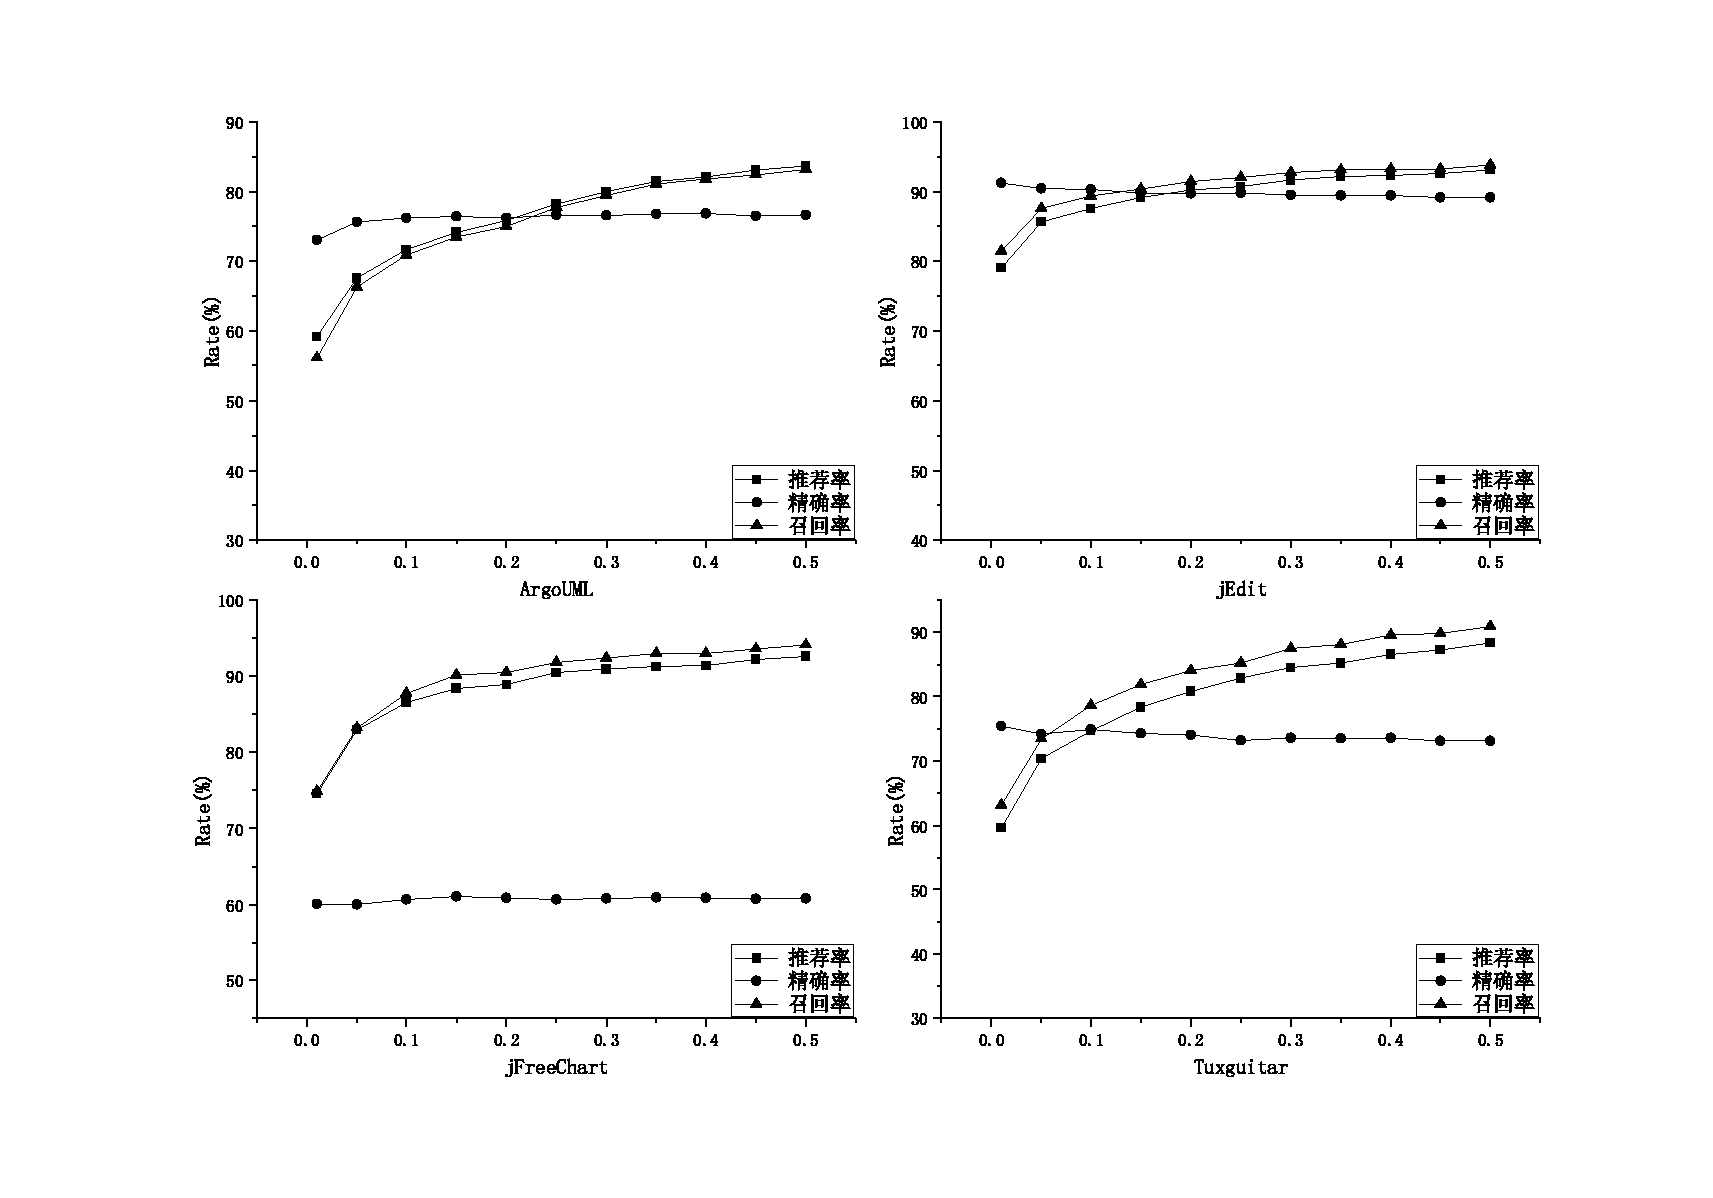
\includegraphics[width = 1.0\textwidth]{bayesgraph/creatingcrossfree.pdf}
\bicaption[creatingcrossfree]{}{克隆创建实例的跨项目使用模式实验结果(不需维护)}
{Fig.$\!$}{The effectiveness of cross-project for usage on meeting creating consistency-free}
\vspace{-1em}
\end{figure}

通过对比四个实验系统的实验结果,不同系统的预测效果不是一致的。发现jEdit系统的预测效果最好,其精确率在89.1\% - 91.2\%之间,召回率在81.4\% - 93.8\%之间。而对jFreeChart系统的预测效果最差,其精确率仅在60\%左右,召回率可以达到90\%以上。而系统ArgoUML和Tuxguitar的预测效果差不多,精确率在75\%左右,召回率最高分别可达76.6\%和90.84\%。分析原因可能是由于jEdit系统的训练集规模最大,模型训练最充分,而jFreeChart则与之相反。

与此同时,贝叶斯网络的阈值会影响预测效果。从图中可以看出,当阈值接近于0.5时,跨项目的预测效果好,系统ArgoUML的精确率和召回率分别为76.6\%和83.1\%,jEdit为89.1\%和93.4\%,jFreeChart为60.8\%和94.8\%,Tuxguitar为73.1\%和90.8\%。

在软件开发初期,当自身系统训练数据较少不足以训练模型的情况下,可以使用其它系统的数据对不需要一致性维护的克隆创建实例进行跨项目预测。所构建模型的预测能力会依赖于项目自身的特征,建议优先选用系统自身的数据进行一致性维护需求预测。同时,建议开发人员调整合适的阈值以达到最佳的预测效果。

%%%%表~\ref{copycrossfreebaysian}~和~\ref{copycrossmeetingbaysian}所示。
%%%%对于克隆创建实例,由统计结果可以看出(~表\ref{instancesta}~),系统中大部分的实例都是不需要进行一致性维护的克隆实例,其比例为59.80-88.47\%。对其进行跨项目一致性预测,其预测结果如表~\ref{copycrossfreebaysian}~所示。

%%%%%从表中可以看出,四个系统的精确率和召回率依然达到了较高的水平,其中精确率在60.01\%--91.20\%之间,召回率56.06\%--91.43\%之间。同时,通过对比发现jEdit的预测效果最好(精确率较高),而jFreeChart预测效果最差。分析原因可能是由于jEdit系统的训练集最大,模型训练最充分,而jFreeChart则与之相反。
%%%%%
%%%%%将实验结果与第3章的全属性实验进行对比(表~\ref{copyallfree}~),可以发现四个系统的预测效果都有了不同程度的下降,但是目跨项目的预测效果依然是可以接受的。
%%%%%
%%%%%因此,预测模型的预测能力会依赖于自身系统数据,建议优先选用系统自身的数据进行一致性为需求预测;在软件开发初期,自身系统训练数据较少,而不足以较好的训练模型的情况下,可以使用其它系统的数据对模型进行跨项目预测。
%%%%%
%%%%%\begin{table}[htbp]
%%%%%\bicaption[copycrossfreebaysian]{}{克隆创建的贝叶斯网络跨项目预测实验结果(不需维护)}
%%%%%{Table$\!$}{The effectiveness for cross-project with Bayesian network at creating time(free)}
%%%%%\vspace{0.5em}
%%%%%\centering
%%%%%\wuhao
%%%%%\begin{tabular}{ccccc}
%%%%%\toprule[1.5pt]
%%%%%{测试系统}&{阈值}&{推荐率(\%)}&{精确率(\%)}&{召回率(\%)}\\
%%%%%\midrule[1pt]
%%%%%\multirow{5}{*}{ArgoUML}
%%%%%&0.01&	59.16&	73.03&	56.06\\
%%%%%&0.05&	67.57&	75.59&	66.28\\
%%%%%&0.10&	71.95&	76.28&	71.21\\
%%%%%&0.15&	74.10&	76.40&	73.47\\
%%%%%&0.20&	75.81&	76.18&	74.94\\
%%%%%\hline
%%%%%\multirow{5}{*}{jEdit}
%%%%%&0.01&	78.99&	91.20&	81.43\\
%%%%%&0.05&	85.62&	90.41&	87.50\\
%%%%%&0.10&	87.52&	90.25&	89.29\\
%%%%%&0.15&	89.10&	89.72&	90.36\\
%%%%%&0.20&	90.21&	89.67&	91.43\\
%%%%%\hline
%%%%%\multirow{5}{*}{jFreeChart}
%%%%%&0.01&	74.48&	60.07&	74.81\\
%%%%%&0.05&	82.92&	60.01&	83.21\\
%%%%%&0.10&	86.51&	60.65&	87.73\\
%%%%%&0.15&	88.38&	61.01&	90.16\\
%%%%%&0.20&	88.92&	60.84&	90.46\\
%%%%%\hline
%%%%%\multirow{5}{*}{Tuxguitar}
%%%%%&0.01&	59.55&	75.44&	63.19\\
%%%%%&0.05&	70.40&	74.16&	73.43\\
%%%%%&0.10&	74.74&	74.91&	78.74\\
%%%%%&0.15&	78.38&	74.29&	81.89\\
%%%%%&0.20&	80.76&	74.00&	84.06\\
%%%%%\bottomrule[1.5pt]
%%%%%\end{tabular}
%%%%%\end{table}

(2)一致性维护需求实验

对于需要一致性维护的克隆创建实例,其跨项目的实验结果如图~\ref{creatingcrossmeeting}所示。从图中可以看出,四个系统的预测效果都比较差。其中,系统ArgoUML的精确率在7.9\% - 20.7\%之间,jEdit的精确率略好,在20.5\% - 75.0\%之间,系统jFreeChart在33.3\% - 52.6\%之间,系统Tuxguitar为44.3\% - 51.9\%。而所有系统的召回率均低于18\%。分析原因是需要维护的克隆创建实例往往会依赖于具体的系统,同时克隆创建实例的样本也不平衡,由统计结果可以看出(~表\ref{instancesta}~),系统中仅有少量的实例满足一致性维护需求,其比例为11.5\% - 40.2\%。因此,所训练的跨项目模型,无法实际的预测需要一致性维护的克隆创建实例。

\begin{figure}[h]
\centering
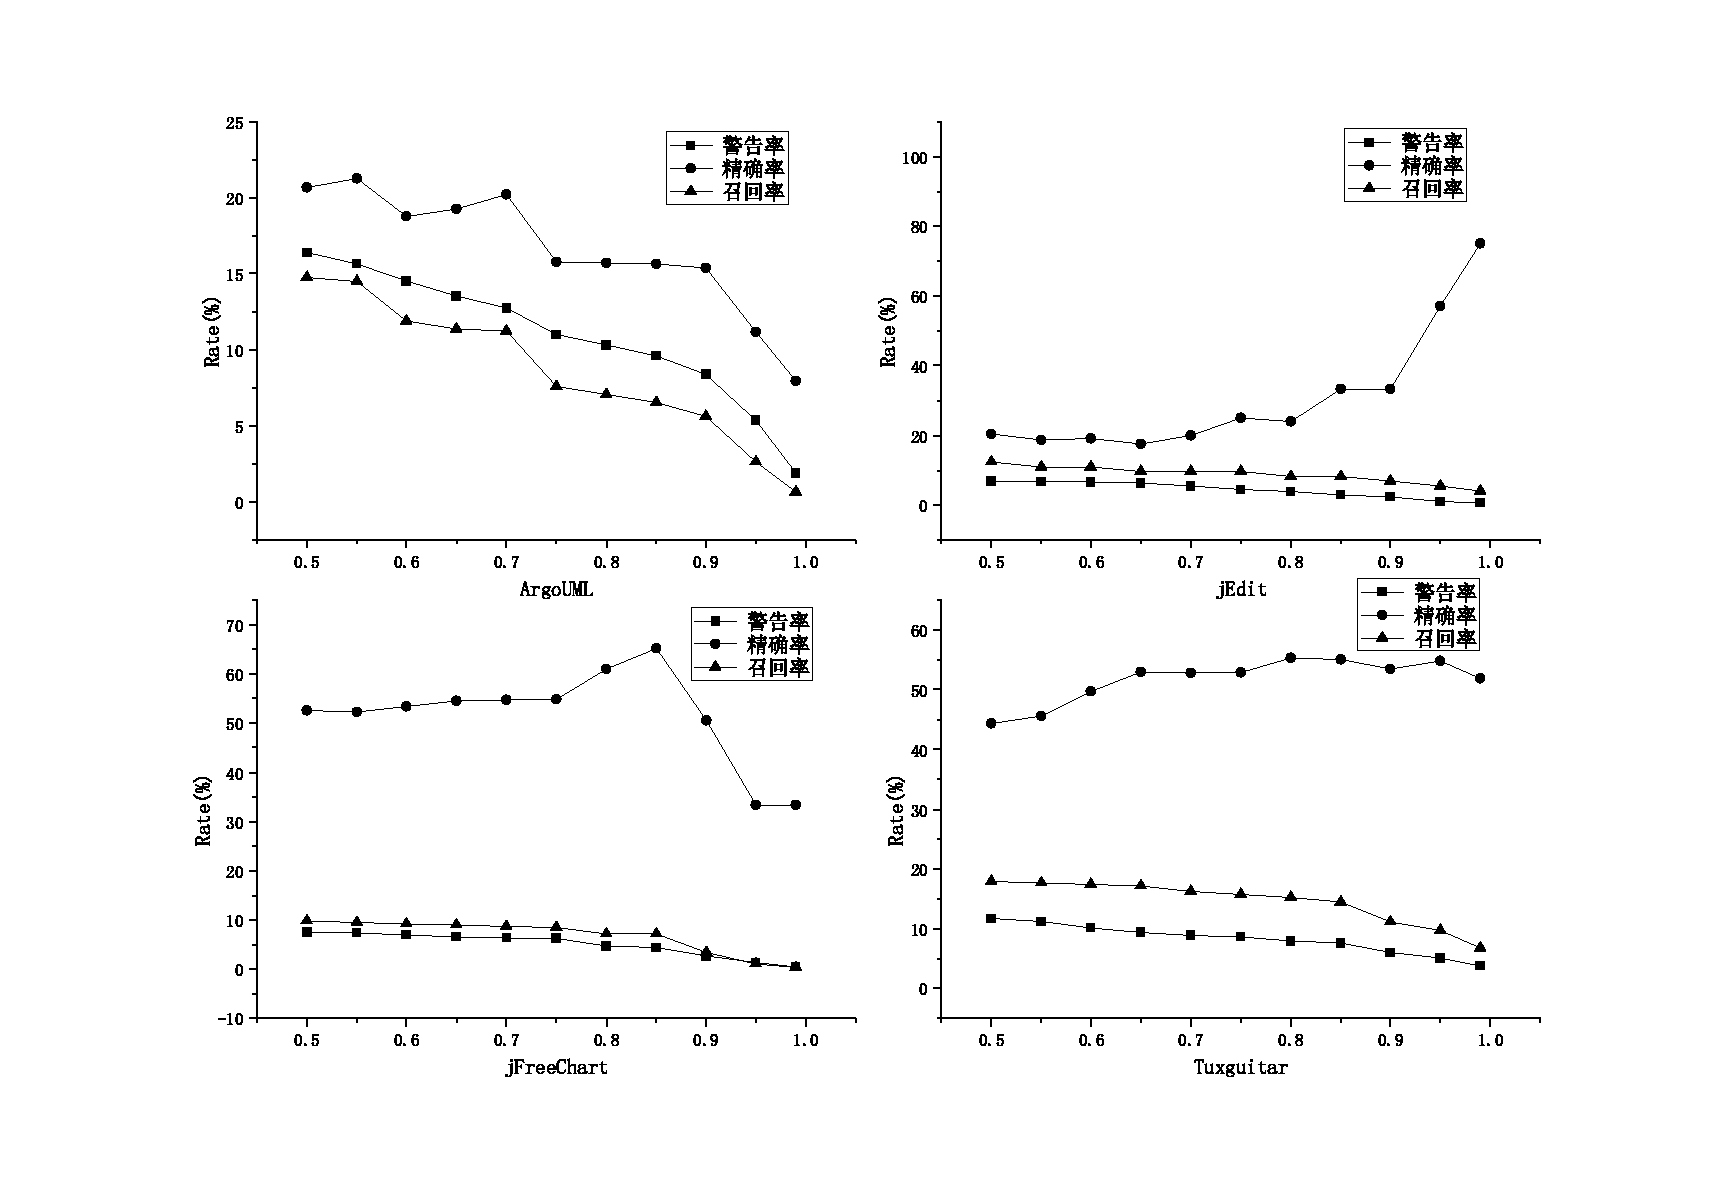
\includegraphics[width = 1.0\textwidth]{bayesgraph/creatingcrossmeeting.pdf}
\bicaption[creatingcrossmeeting]{}{克隆创建实例的跨项目使用模式实验结果(需要维护)}
{Fig.$\!$}{The effectiveness of cross-project for usage on meeting creating consistency}
\vspace{-1em}
\end{figure}

同时,与第3章全属性实验进行对比(图~\ref{creatingallmeeting}~),发现四个系统的跨项目预测效果下降得十分严重。因此,对需要一致性维护的克隆创建实例,强烈的依赖于具体的系统,不建议使用跨项目的方式对其进行一致性维护需求预测。

因此, 对于需要一致性维护的克隆创建实例,本文不建议使用跨项目的方式对需要一致性维护需求预测。原因可能是由于克隆代码的一致性变化往往会依赖于具体的系统的特征,而跨项目之间的差异无法较好的训练相应的模型,因此建议开发人员选择自身数据进行训练和预测。在开发初期由于缺乏数据问题无法训练相应模型时,建议程序开发人员选择对不需要一致性维护的克隆实例进行跨项目预测。

%%%%原表格
%%%%%对于克隆创建实例,由统计结果可以看出(~表\ref{instancesta}~),系统中仅有少量的实例满足一致性维护需求,其比例为11.53-40.20\%。对其进行跨项目一致性预测,实验结果如~\ref{copycrossmeetingbaysian}所示。
%%%%%
%%%%%从表中可以看出,四个系统的预测效果都比较差,精确率在15.36\%--61.01\%之间,召回率则更低,仅在10\%徘徊。分析原因是克隆创建实例的样本不平衡,其中大部分的数据是不需要一致性维护。所以,所训练的模型不够完善,跨项目预测能力无法达到实际应用的水平。
%%%%%
%%%%%与第3章全属性实验进行对比(表~\ref{copyallmeeting}~),发现四个系统的跨项目预测效果下降的均十分严重。因此,对需要一致性维护的克隆创建实例,不建议使用跨项目的方式进行克隆一致性预测。
%%%%%
%%%%%因此, 对于需要一致性维护的克隆创建实例,本文同样不建议使用跨项目的方式对需要一致性维护的克隆创建实例进行预测,而是选择自身数据进行预测。在开发初期由于缺乏数据问题,建议程序开发人员选择对不需要的克隆实例进行预测。
%%%%%
%%%%%\begin{table}[htbp]
%%%%%\bicaption[copycrossmeetingbaysian]{}{克隆创建的贝叶斯网络方法跨项目预测实验结果(需要维护)}
%%%%%{Table$\!$}{The effectiveness for cross-project with Bayesian network at creating time(meeting)}
%%%%%\vspace{0.5em}
%%%%%\centering
%%%%%\wuhao
%%%%%\begin{tabular}{ccccc}
%%%%%\toprule[1.5pt]
%%%%%{测试系统}&{阈值}&{警告率(\%)}&{精确率(\%)}&{召回率(\%)}\\
%%%%%\midrule[1pt]
%%%%%\multirow{5}{*}{ArgoUML}
%%%%%&0.90&	8.38&	15.36&	5.61\\
%%%%%&0.80&	10.30&	15.70&	7.05\\
%%%%%&0.70&	12.75&	20.19&	11.23\\
%%%%%&0.60&	14.52&	18.76&	11.88\\
%%%%%&0.50&	16.38&	20.66&	14.75\\
%%%%%\hline
%%%%%\multirow{5}{*}{jEdit}
%%%%%&0.90&	2.37&	33.33&	6.85\\
%%%%%&0.80&	3.95&	24.00&	8.22\\
%%%%%&0.70&	5.53&	20.00&	9.59\\
%%%%%&0.60&	6.64&	19.05&	10.96\\
%%%%%&0.50&	6.95&	20.45&	12.33\\
%%%%%\hline
%%%%%\multirow{5}{*}{jFreeChart}
%%%%%&0.90&	2.70&	50.55&	3.40\\
%%%%%&0.80&	4.72&	61.01&	7.17\\
%%%%%&0.70&	6.36&	54.67&	8.65\\
%%%%%&0.60&	6.95&	53.42&	9.24\\
%%%%%&0.50&	7.46&	52.59&	9.76\\
%%%%%\hline
%%%%%\multirow{5}{*}{Tuxguitar}
%%%%%&0.90&	6.02&	53.49&	11.14\\
%%%%%&0.80&	7.98&	55.26&	15.25\\
%%%%%&0.70&	8.89&	52.76&	16.22\\
%%%%%&0.60&	10.15&	49.66&	17.43\\
%%%%%&0.50&	11.69&	44.31&	17.92\\
%%%%%\bottomrule[1.5pt]
%%%%%\end{tabular}
%%%%%\end{table}

(3)小结

综上,针对克隆创建实例的跨项目预测,实验结果表明所构建的预测模型的有效性会依赖于系统自身的某些特征。因此,本文建议优先选用自身的数据进行模型训练和和预测。

在软件开发初期,当自身系统的数据太少而不足以训练模型时,可以使用跨项目预测的方式,对不需要一致性维护的克隆创建实例进行预测,仅仅允许此类的克隆实例产生,从而避免额外的一致性维护代价。由于系统具有较少的需要一致性维护的克隆创建实例,并且会依赖于具体系统的某些特征,对需要一致性维护的克隆创建实例的预测效果较差。因此,本文不建使用跨项目的方式对其进行一致性维护需求预测。

\BiSubsubsection{克隆变化实例的实验结果}
{The Results for Clone Changing Instances}

本节对克隆变化实例进行跨项目一致性维护需求预测,在四个系统上对两种状态的变化实例的实验结果分别如图~\ref{changingcrossfree}~和图~\ref{changingcrossmeeting}所示。

(1)一致性维护自由实验

对不需要一致性维护的克隆变化实例,其跨项目一致性预测结果如图~\ref{changingcrossfree}~所示。

\begin{figure}[h]
\centering
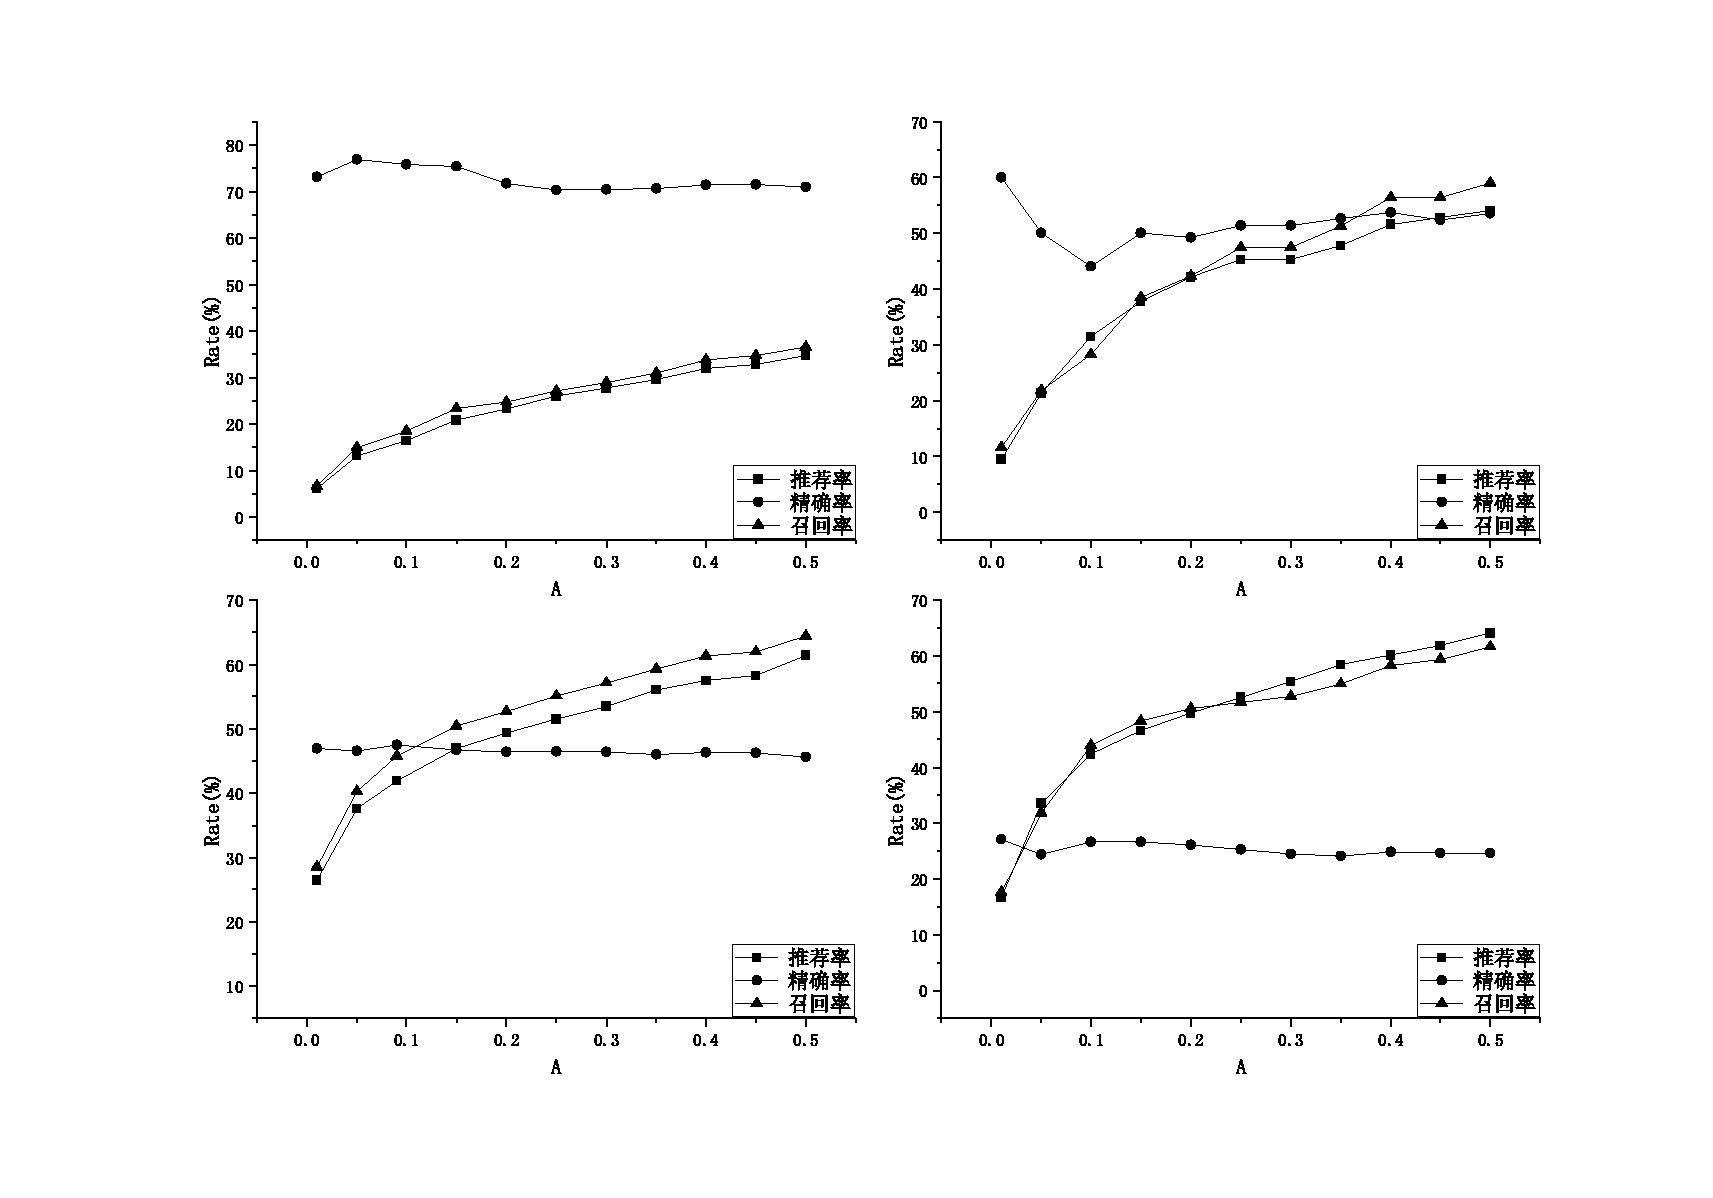
\includegraphics[width = 1.0\textwidth]{bayesgraph/changingcrossfree.pdf}
\bicaption[changingcrossfree]{}{克隆变化实例的跨项目使用模式实验结果(不需维护)}
{Fig.$\!$}{The effectiveness of cross-project for usage on meeting changing consistency-free}
\vspace{-1em}
\end{figure}

从图中可以看出,跨项目预测在四个系统上预测效果较为一般。ArgoUML系统的精确率最好,达到了70.3\%以上,系统jEdit和jFreeChart的精确率在50\%左右,而系统Tuxguitar的预测效果最差,仅在25\%左右。同时,四个系统的召回率并不能令人满意。其中,系统ArgoUML的召回率最低(低于36.46\%),其它系统的召回率最高可以达到60\%左右。分析原因可能是克隆代码的变化情况较高的依赖于具体的系统的数据分布情况。

结合第4章项目内的预测结果(图~\ref{changingallfree}~),可以发现当使用自身系统的数据作为训练集且训练集足够大时,预测模型有效的。因此,本文建议使用系统自身的数据进行一致性维护需求预测。采用跨项目预测的情况下,所构建的模型无法较好地预测不需要一致性维护的克隆变化实例。

跨项目预测的效果是较为稳定的,阈值变化会影响到预测的效果,其中对召回率的影响大于对精确率的影响。从图中可以看出,推荐率和召回率具有正相关的关系,并受阈值的影响较大。跨项目预测的精确率与具体的系统有关,预测效果是较为稳定的,即精确率稳定在一个稳范围内。随着阈值的升高,所推荐的不需要克隆变化实例的数量变多,因而导致召回率的提高。

因此,在软件开发的初期阶段,由于缺乏足够数量的克隆变化实例,不能很好地训练模型时,开发人员可以使用本文第3章提出的方法在克隆创建时预测克隆代码的一致性,从而仅允许那些不需要一致性维护的克隆实例产生。在软件演化到了足够的版本时,随着来自其自己的克隆变化数据的增加,开发人员可以使用自身数据重新训练模型以预测项目中克隆变化的一致性维护需求。

%%%本节给出在克隆代码变化时,四个系统上的实验结果如表~\ref{changecrossfreebaysian}~和~\ref{changecrossmeetingbaysian}所示。
%%%%对不需要一致性维护的克隆变化实例,跨项目一致性预测结果如表~\ref{changecrossfreebaysian}~所示。从表中可以看出,ArgoUML的精确率最好,达71.72\%以上,系统jEdit和jFreeChart的预测效果在50\%左右,而Tuxguitar的预测效果最差。结合数据的不平衡性,发现预测效果向需要一致性维护的实例偏移。因此,精确度预测效果与样本自身的特征有关联关系,即最好选择向数据较多的一侧进行预测。同时,四个系统的召回率都不尽如意,未能达到较好的预测效果。分析原因,是由于样本之间具有较大的差异,跨项目数据无法较好的拟合被测试系统的样本数据。
%%%%
%%%%结合全属性实验的实验结果(表~\ref{changeallfree}~),可以发现当使用自身系统的数据作为训练集且训练集足够大时,预测模型有效的。因此,本文建议使用系统自身的数据进行一致性预测,不建议使用跨项目的形式进行预测。
%%%%
%%%%然而,在软件开发的初期阶段,由于缺乏足够数量的克隆变化实例,不能很好的训练模型时,开发人员可以使用本文第3章提出的方法在克隆创建时预测克隆代码的一致性,从而仅允许那些不需要一致性维护的克隆实例产生。在软件演化到了足够的版本时,随着来自其自己的克隆变化数据的增加,开发人员可以使用自身数据重新训练模型以预测项目中克隆变化的一致性维护需求。
%%%%
%%%%\begin{table}[htbp]
%%%%\bicaption[changecrossfreebaysian]{}{克隆变化的贝叶斯网络方法跨项目预测实验结果(不需维护)}
%%%%{Table$\!$}{The effectiveness for cross-project with Bayesian network at changing time(free)}
%%%%\vspace{0.5em}
%%%%\centering
%%%%\wuhao
%%%%\begin{tabular}{ccccc}
%%%%\toprule[1.5pt]
%%%%{测试系统}&{阈值}&{推荐率(\%)}&{精确率(\%)}&{召回率(\%)}\\
%%%%\midrule[1pt]
%%%%\multirow{5}{*}{ArgoUML}
%%%%&0.01&	6.09&	73.08&	6.60\\
%%%%&0.05&	13.11&	76.79&	14.93\\
%%%%&0.1&	16.63&	74.65&	18.40\\
%%%%&0.15&	20.84&	75.28&	23.26\\
%%%%&0.2&	23.19&	71.72&	24.65\\
%%%%\hline
%%%%\multirow{5}{*}{jEdit}
%%%%&0.01&	9.43&	60.00&	11.54\\
%%%%&0.05&	21.38&	50.00&	21.79\\
%%%%&0.1&	31.45&	44.00&	28.21\\
%%%%&0.15&	37.74&	50.00&	38.46\\
%%%%&0.2&	42.14&	49.25&	42.31\\
%%%%\hline
%%%%\multirow{5}{*}{jFreeChart}
%%%%&0.01&	26.44&	46.91&	28.54\\
%%%%&0.05&	37.60&	46.55&	40.27\\
%%%%&0.1&	43.27&	47.56&	47.35\\
%%%%&0.15&	46.92&	46.72&	50.44\\
%%%%&0.2&	49.33&	46.39&	52.65\\
%%%%\hline
%%%%\multirow{5}{*}{Tuxguitar}
%%%%&0.01&	16.67&	27.12&	17.58\\
%%%%&0.05&	33.62&	24.37&	31.87\\
%%%%&0.1&	42.37&	26.67&	43.96\\
%%%%&0.15&	46.61&	26.67&	48.35\\
%%%%&0.2&	49.72&	26.14&	50.55\\
%%%%\bottomrule[1.5pt]
%%%%\end{tabular}
%%%%\end{table}

(2)一致性维护需求实验

对需要一致性维护的克隆变化实例,跨项预测的实验结果如图~\ref{changingcrossmeeting}~所示。

\begin{figure}[h]
\centering
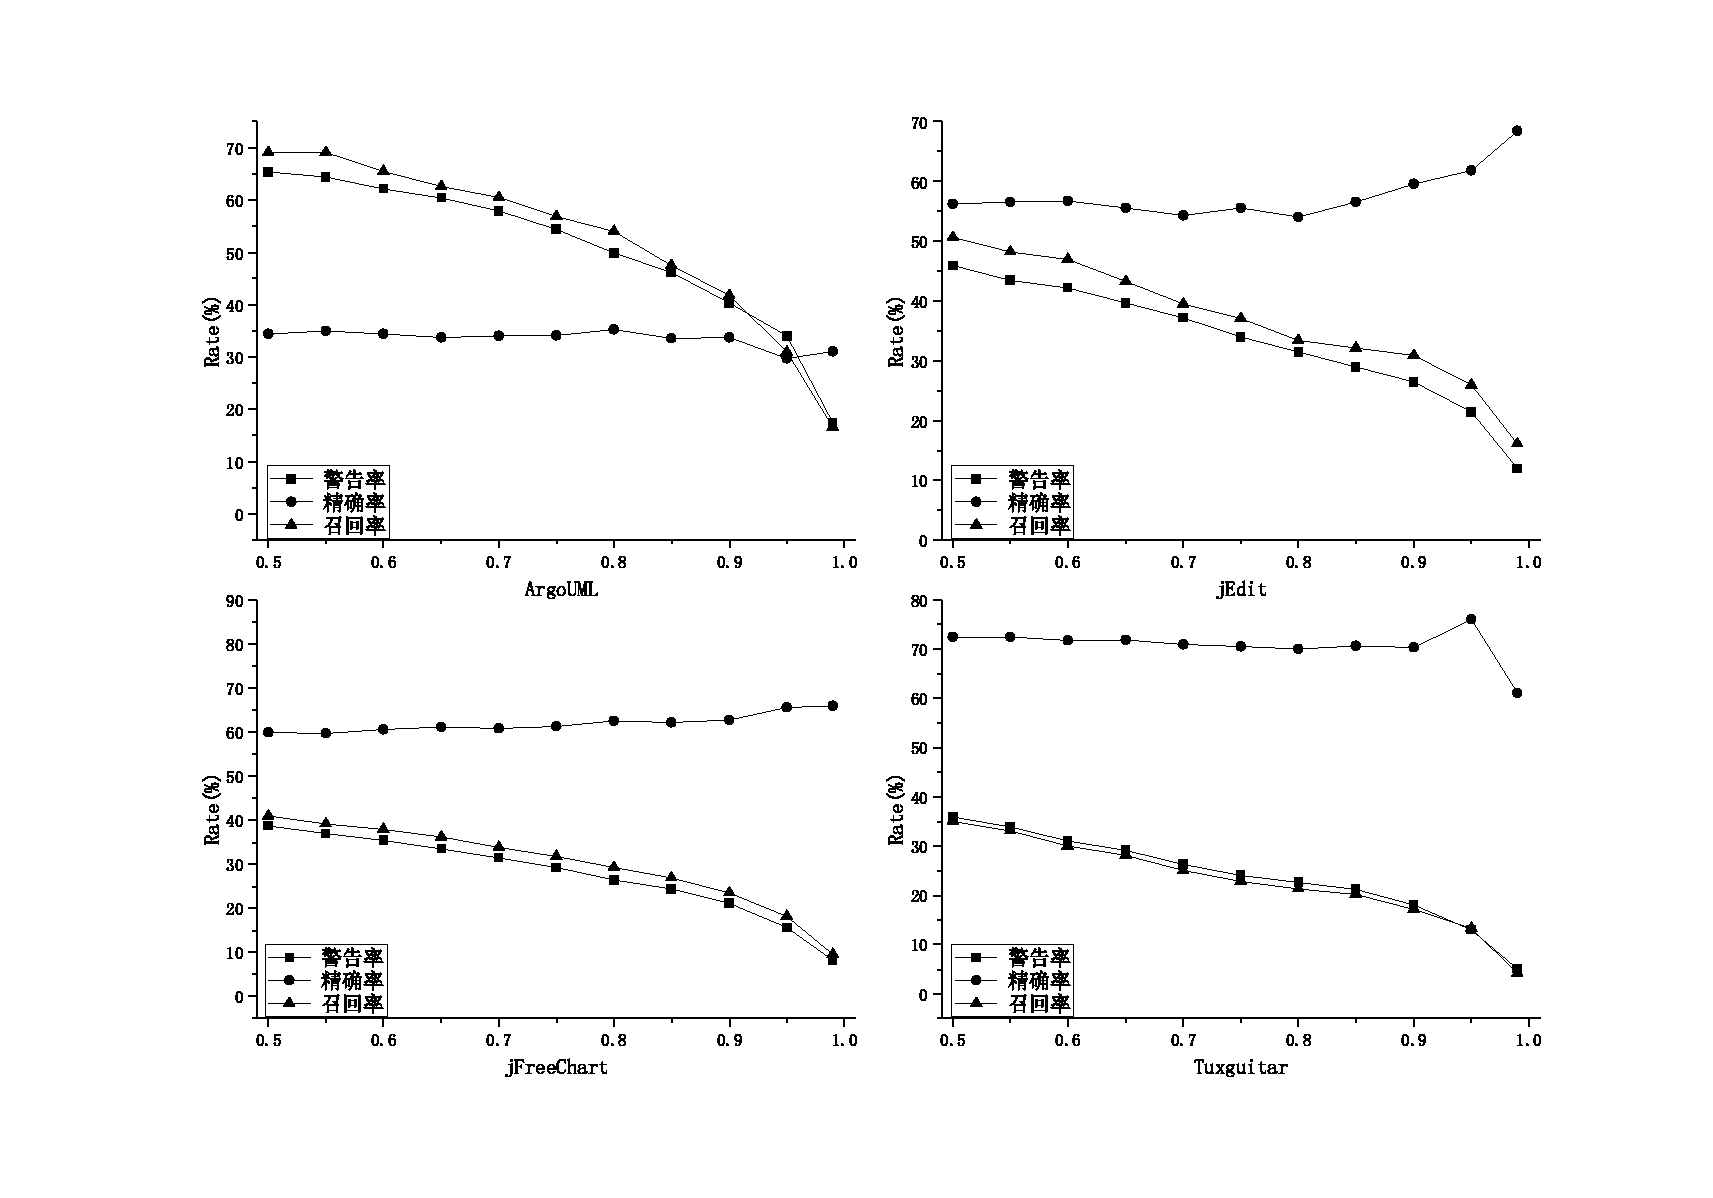
\includegraphics[width = 1.0\textwidth]{bayesgraph/changingcrossmeeting.pdf}
\bicaption[changingcrossmeeting]{}{克隆变化实例的跨项目使用模式实验结果(需要维护)}
{Fig.$\!$}{The effectiveness of cross-project for usage on meeting changing consistency}
\vspace{-1em}
\end{figure}

从图中可以看出,对需要一致性维护的克隆变化实例,预测效果也较为一般。Tuxguitar系统的精确率最好,在70\%左右,系统jEdit和jFreeChart的预测效果在60\%左右,而Tuxguitar的预测效果最差,仅在30\%左右。同时对于召回率来说,系统Tuxguitar和jFreeChart的召回率最低,最高分别可以达到30\%和40\%左右。jEdit和ArgoUML的召回率较好,分别可以达到50\%和70\%左右。结合全属性实验的实验结果(图~\ref{changingallmeeting}~),可以发现当使用自身系统的数据作为训练集且训练集足够大时,预测模型有效的。因此,本文建议优先使用系统自身的数据进行一致性预测,当数据不足以预测自身项目时,再使用跨项目的形式进行预测。

跨项目预测的效果是较为稳定的,阈值变化会影响到预测的效果,其中对召回率的影响大于对精确率的影响。从图中可以看出,推荐率和召回率具有正相关的关系,并受阈值的影响较大。跨项目预测的预测效果是较为稳定的,即精确率稳定在一个稳范围内。跨项目预测的精确率与具体的系统有关。随着阈值的升高,所推荐的不需要克隆变化实例的数量变多,因而导致召回率的升高。

在软件开发的初期阶段,由于缺乏足够数量的克隆变化实例,建议开发人员使用本文第3章提出的方法在克隆创建时预测克隆代码的一致性,从而仅允许那些不需要一致性维护的克隆实例产生。在软件演化到了足够的版本时,随着来自其自己的克隆变化数据的增加,开发人员可以使用自身数据重新训练模型以预测项目中克隆变化的一致性。

%%%%对需要一致性维护的克隆变化实例,跨项目一致性预测结果如表~\ref{changecrossmeetingbaysian}~所示。
%%%%
%%%%从表中可以看出,Tuxguitar的精确率最好,达70\%以上,系统jEdit和jFreeChart的预测效果在60\%左右,而Tuxguitar的预测效果最差,仅在33\%左右。结合数据的不平衡性,发现预测效果向需要一致性维护的实例偏移。因此,精确度预测效果与样本自身的特征有关联关系,即最好选择向数据较多的一侧进行预测。同时,四个系统的召回率都不尽如意,未能达到较好的预测效果。分析原因,是由于样本之间具有较大的差异,跨项目数据无法较好的拟合被测试系统的样本数据。
%%%%
%%%%结合全属性实验的实验结果(表~\ref{changeallmeeting}~),可以发现当使用自身系统的数据作为训练集且训练集足够大时,预测模型有效的。因此,本文建议优先使用系统自身的数据进行一致性预测,当数据不足以预测自身项目时,可以使用跨项目的形式进行预测。
%%%%
%%%%同时,在软件开发的初期阶段,由于缺乏足够数量的克隆变化实例,不能很好的训练模型时,开发人员依然可以使用本文第3章提出的方法在克隆创建时预测克隆代码的一致性,从而仅允许那些不需要一致性维护的克隆实例产生。在软件演化到了足够的版本时,随着来自其自己的克隆变化数据的增加,开发人员可以使用自身数据重新训练模型以预测项目中克隆变化的一致性。
%%%%
%%%%\begin{table}[htbp]
%%%%\bicaption[changecrossmeetingbaysian]{}{克隆变化的贝叶斯网络方法跨项目预测实验结果(需要维护)}
%%%%{Table$\!$}{The effectiveness for cross-project with Bayesian network at changing time(meeting)}
%%%%\vspace{0.5em}
%%%%\centering
%%%%\wuhao
%%%%\begin{tabular}{ccccc}
%%%%\toprule[1.5pt]
%%%%{测试系统}&{阈值}&{警告率(\%)}&{精确率(\%)}&{召回率(\%)}\\
%%%%\midrule[1pt]
%%%%\multirow{5}{*}{ArgoUML}
%%%%&0.9&	40.28&	33.72&	41.73\\
%%%%&0.8&	49.88&	35.21&	53.96\\
%%%%&0.7&	57.85&	34.01&	60.43\\
%%%%&0.6&	62.06&	34.34&	65.47\\
%%%%&0.5&	65.34&	34.41&	69.06\\
%%%%\hline
%%%%\multirow{5}{*}{jEdit}
%%%%&0.9&	26.42&	59.52&	30.86\\
%%%%&0.8&	31.45&	54.00&	33.33\\
%%%%&0.7&	37.11&	54.24&	39.51\\
%%%%&0.6&	42.14&	56.72&	46.91\\
%%%%&0.5&	45.91&	56.16&	50.62\\
%%%%\hline
%%%%\multirow{5}{*}{jFreeChart}
%%%%&0.9&	21.15&	62.73&	23.47\\
%%%%&0.8&	26.44&	62.55&	29.25\\
%%%%&0.7&	31.44&	60.86&	33.84\\
%%%%&0.6&	35.38&	60.60&	37.93\\
%%%%&0.5&	38.65&	59.95&	40.99\\
%%%%\hline
%%%%\multirow{5}{*}{Tuxguitar}
%%%%&0.9&	18.08&	70.31&	17.11\\
%%%%&0.8&	22.60&	70.00&	21.29\\
%%%%&0.7&	26.27&	70.97&	25.10\\
%%%%&0.6&	31.07&	71.82&	30.04\\
%%%%&0.5&	35.88&	72.44&	34.98\\
%%%%\bottomrule[1.5pt]
%%%%\end{tabular}
%%%%\end{table}

(3)小结

对于克隆变化实例,实验表明跨项目预测模型的有效性会依赖于系统自身的某些特征。本文建议开发人员优先选用自身的数据进行模型训练,以达到满意的预测效果。

在软件开发初期阶段,由于自身系统的数据太少而不足以训练模型时,跨项目预测效果(精确率)将依赖于数据集的分布情况。对于被测试的软件系统,需要尽量选择那些具有相似数据分布的测试系统,训练模型进行跨项目预测。以本文使用的实验系统为例,对于其中三个系统,其需要维护的克隆变化实例较多,因此所训练的跨项目模型,在需要一致性维护的预测中预测效果要优于不需要维护的预测。

同时,在软件开发初期,系统自身缺乏克隆变化实例而无法构建预测模型。当跨项目的模型也无法使用时,建议开发人员使用本文第3章的方法,在克隆代码创建时进行一致性维护需求预测,尽量避免会导致一致性变化的克隆代码。

\BiSubsubsection{讨论}
{Discussion}

综上所述,可以回答第二个研究子问题:

首先,由于项目之间的差异性,测试集和训练集也具有较大差异,跨项目预测能力达不到项目内预测的能力。因此,建议开发人员优先选择项目内的预测方式。

其次,在软件开发初期,由于缺乏系统自身的数据而无法训练机器学习模型时,可以使用跨项目方式进行克隆一致性维护需求预测,帮助避免由于克隆代码所导致的维护代价。但由于训练数据的样本不平衡性,跨项目预测能力会向数据较多的一侧倾斜,因此建议选择数据较多的一个角度进行预测:(1)在克隆代码创建时,建议对不需要一致性维护的克隆实例进行预测,帮助快速的执行复制和粘贴操作。(2)克隆代码变化时,建议对需要一致性维护的克隆实例进行预测,帮助避免克隆一致性维护缺陷。

最后,在进行选择跨项目预测时,软件开发人员可以根据自身需求,选择具有相似分布的训练系统,以达到较好的预测效果。如何选择相似的系统,将是本文未来的研究工作。


\BiSubsection{跨项目训练集规模实验}
{The Experiments of Cross-Project Prediction for Training Size}

在进行克隆代码一致性维护需求预测时,训练集的规模会影响预测效果。为了探索数据集规模对预测效果的影响,本节实验使用不同的训练集训练模型,并预测克隆代码的一致性维护需求。并回答本章提出的第三个研究问题:在进行跨项目的克隆一致性维护需求预测时,训练数据的规模将如何影响跨项目的克隆一致性维护需求的预测效果?

在五种机器学习方法上进行了跨项目的数据集规模实验,并使用平均精确率(Average Precision)、平均召回率(Average Recall)和平均F值(Average F-measure)进行评价(见本文第~\ref{ref-creatingmetrics}~节和第~\ref{ref-changingmetrics}~节)。

首先,进行“一对一”跨项目预测。“一对一”跨项目预测是指每次仅使用一个系统的数据作为训练集,在目标系统上进行跨项目预测,并对多个训练系统的预测结果进行平均,得出“一对一”的预测结果(使用“Average”表示,简写为Ave)。然后,进行“多对一”跨项目预测。“多对一”跨项目预测是指使用三个系统的数据集共同作为训练集,并在目标系统上进行跨项目预测,得出多对一预测结果(使用“All”表示)。最后,进行“数据集扩大”实验,新增三个不同实验系统扩大跨项目预测的训练集(使用“Expansion”表示,简写为Exp)。扩大训练集所采用的系统为DNSjava、Carol和JabRef三个实验系统。其中,选择了34个软件版本的DNSjava系统,11个版本的Carol系统和19个版本的JabRef系统。

对克隆创建实例和变化实例进行了实验评估,实验结果如表~\ref{creatingcrosssizeaverage}~和表~\ref{changingcrosssizeaverage}~所示。表中“Precision”、“Recall”、“F-measure”分别指平均精确率、平均召回率和平均F值。



\BiSubsubsection{克隆创建实例的实验结果}
{The Results for Clone Creating Instances}

对克隆创建实例进行跨项目预测,实验结果如表~\ref{creatingcrosssizeaverage}~所示,其中“All”列表示“多对一”实验结果,“Ave”列表示“一对一”实验结果,“Exp”列表示扩大数据集实验结果。

\begin{table} [h]
\bicaption[creatingcrosssizeaverage]{}{克隆创建实例的跨项目数据集规模实验结果}
{Table$\!$}{The effectiveness of cross-project for training size on creating instances}
\vspace{0.5em}
\centering
\footnotesize
\begin{tabular}{cccccccccccccc}
\toprule[1.5pt]
~\multirow{2}{*}{指标}&\multirow{2}{*}{方法}&\multicolumn{3}{c}{To ArgoUML}&\multicolumn{3}{c}{To jEdit}&\multicolumn{3}{c}{To jFreeChart}&\multicolumn{3}{c}{To  Tuxguitar}\\
\cline{3-14}
~&~&{Ave}&{All}&{Exp}&{Ave}&{All}&{Exp}&{Ave}&{All}&{Exp}&{Ave}&{All}&{Exp}\\
\midrule[1pt]
\multirow{5}{*}{Precision(\%)}
&BN&63.3&63.8&61.8&81.0&81.2&79.6&55.6&57.5&57.0&63.3&64.8&60.7\\
&NB&62.9&63.1&66.4&79.2&78.3&78.5&50.2&48.6&52.3&60.6&61.5&54.8\\
&SVM&65.7&59.4&62.8&78.3&78.3&78.2&35.8&35.8&41.0&50.6&50.6&60.0\\
&KNN&62.9&62.9&60.1&81.5&78.6&78.0&	61.7&64.8&49.6&58.7&58.1&56.7\\
&DT&68.6&62.9&62.1&78.2&79.6&81.6&	53.0&56.6&42.1&59.4&70.4&54.1\\
\hline
\multirow{5}{*}{Recall(\%)}															
&BN&67.0&67.5&68.7&75.2&84.4&80.3&60.6&60.2&60.0&67.4&69.8&64.2\\
&NB&66.9&69.3&57.7&75.4&74.7&49.1&56.4&54.0&44.5&64.3&64.7&48.6\\
&SVM&80.9&77.1&72.1&88.5&88.5&88.2&59.8&59.8&59.2&71.1&71.1&70.2\\
&KNN&68.1&68.7&62.2&76.2&74.1&71.7&63.5&64.9&55.2&65.5&66.3&62.8\\
&DT	&76.4&74.0&66.7&80.3&84.4&70.8&59.5&59.9&50.2&68.8&73.1&56.8\\
\hline
\multirow{5}{*}{F-measure(\%)}					
&BN&64.5&65.4&64.7&76.8&82.6&79.9&51.6&50.8&51.5&63.1&65.0&62.0\\
&NB&64.5&65.6&60.7&77.4&76.4&58.0&48.8&48.9&40.0&61.7&62.7&50.8\\
&SVM&72.4&67.1&66.3&83.1&83.1&82.9&44.8&44.8&44.7&59.1&59.1&60.1\\
&KNN&65.1&65.3&61.1&78.1&76.2&74.6&57.9&60.9&49.4&60.1&60.3&58.9\\
&DT	&70.3&66.7&64.1&78.9&81.8&75.1&48.4&50.3&44.1&61.2&68.3&55.3\\
\bottomrule[1.5pt]
\end{tabular}
\end{table}

%%%%未扩大数据集
%%%%\begin{table} [h]
%%%%\bicaption[creatingcrosssizeaverage]{}{克隆创建实例的跨项目数据集规模实验结果}
%%%%{Table$\!$}{The effectiveness of cross-project for training size on creating instances}
%%%%\vspace{0.5em}
%%%%\centering
%%%%\footnotesize
%%%%\begin{tabular}{cccccccccc}
%%%%\toprule[1.5pt]
%%%%~\multirow{2}{*}{指标}&\multirow{2}{*}{方法}&\multicolumn{2}{c}{To ArgoUML}&\multicolumn{2}{c}{To jEdit}&\multicolumn{2}{c}{To jFreeChart}&\multicolumn{2}{c}{To  Tuxguitar}\\
%%%%\cline{3-10}
%%%%~&~&{Average}&{All}&{Average}&{All}&{Average}&{All}&{Average}&{All}\\
%%%%\midrule[1pt]
%%%%\multirow{5}{*}{平均Precision(\%)}
%%%%&BN&63.3&63.8&81.0&81.2&55.6&57.5&63.3&64.8\\
%%%%&NB&62.9&63.1&79.2&78.3&50.2&48.6&60.6&61.5\\
%%%%&SVM&65.7&59.4&78.3&78.3&35.8&35.8&50.6&50.6\\
%%%%&KNN&62.9&62.9&81.5&78.6&	61.7&64.8&58.7&58.1\\
%%%%&DT&68.6&62.9&78.2&79.6&	53.0&56.6&59.4&70.4\\
%%%%\hline
%%%%\multirow{5}{*}{平均Recall(\%)}															
%%%%&BN&67.0&67.5&75.2&84.4&60.6&60.2&67.4&69.8\\
%%%%&NB&66.9&69.3&75.4&74.7&56.4&54.0&64.3&64.7\\
%%%%&SVM&80.9&77.1&88.5&88.5&59.8&59.8&71.1&71.1\\
%%%%&KNN&68.1&68.7&76.2&74.1&63.5&64.9&65.5&66.3\\
%%%%&DT	&76.4&74.0&80.3&84.4&59.5&59.9&68.8&73.1\\
%%%%\hline
%%%%\multirow{5}{*}{平均F-measure(\%)}					
%%%%&BN&64.5&65.4&76.8&82.6&51.6&50.8&63.1&65.0\\
%%%%&NB&64.5&65.6&77.4&76.4&48.8&48.9&61.7&62.7\\
%%%%&SVM&72.4&67.1&83.1&83.1&44.8&44.8&59.1&59.1\\
%%%%&KNN&65.1&65.3&78.1&76.2&57.9&60.9&60.1&60.3\\
%%%%&DT	&70.3&66.7&78.9&81.8&48.4&50.3&61.2&68.3\\
%%%%\bottomrule[1.5pt]
%%%%\end{tabular}
%%%%\end{table}

在数据集规模实验中,“一对一”实验中的每一个系统的训练集规模都是最小的,仅使用一个项目作为训练集。同时,“多对一”预测的实验中训练集规模居中,使用三个项目作为训练集。而“数据集扩大”实验中所使用训练集的规模最大,使用6个项目作为训练集。

首先,对于某一具体的测试系统来说,根据其训练集的规模大小,发现跨项目预测效果和训练集规模并不存在明显的正相关关系,即训练集的大小并不能明显的影响跨项目的预测能力。通过对比同一系统的“Ave”、“All”和“Exp”列,在4个系统中全部的平均F值中,所得到预测结果相差不大。分析其原因,可能是由于在跨项目预测中,项目之间的差异导致所训练的模型不够完善。因此,训练集规模的大小在跨项目预测中不能起到决定性作用。

其次,在预测跨项目的克隆创建实例时,预测效果可能会依赖于某具体的系统。通过对比不同系统的跨项目预测结果,可以发现jEdit系统的实验效果最好,其F值在80\%左右;ArgoUML系统和Tuxguitar系统的跨项目预测效果次之,其F值在60\% - 70\%左右;jFreeChart系统的预测效果最差,F值在50\%左右。因此,在进行跨项目预测时,可以考虑在保证一定规模训练数据的基础上,对训练项目进行进一步的优选,选择与目标项目相似的数据作为训练集,从而缩小项目之间的差异,提升跨项目的预测效果。但是,在跨项目预测中如何对项目进行优选仍需进一步的研究。

%%%%%%\begin{sidewaystable} [htbp]
%%%%%%\bicaption[creatingcrosssizefree]{}{创建时跨项目预测数据集选择实验(free)}
%%%%%%{Table$\!$}{The effectiveness of cross-project for training size selection at creating time(free)}
%%%%%%\vspace{0.5em}
%%%%%%\centering
%%%%%%\wuhao
%%%%%%\begin{tabular}{cccccccccc}
%%%%%%\toprule[1.5pt]
%%%%%%~\multirow{2}{*}{度量}&\multirow{2}{*}{方法}&\multicolumn{2}{c}{To ArgoUML}&\multicolumn{2}{c}{To jEdit}&\multicolumn{2}{c}{To jFreeChart}&\multicolumn{2}{c}{To  Tuxguitar}\\
%%%%%%\cline{3-10}
%%%%%%~&~&{Average}&{All}&{Average}&{All}&{Average}&{All}&{Average}&{All}\\
%%%%%%\midrule[1pt]
%%%%%%\multirow{5}{*}{Precision}
%%%%%%&BN&	0.763&	0.766&	0.887&	0.891&	0.615&	0.608&0.729&	0.731\\
%%%%%%&NB&	0.760&	0.764&	0.880&	0.876&	0.593&	0.584&	0.720	&0.725\\
%%%%%%&SVM&	0.809&	0.771	&0.885&	0.885&	0.598&	0.598&	0.711&	0.711\\
%%%%%%&KNN&	0.762&	0.763	&0.894&	0.878&	0.641&	0.65&	0.709&	0.709\\
%%%%%%&DT	&0.785	&0.767&0.882	&0.885&	0.620	&0.606&	0.718&	0.746\\
%%%%%%\hline
%%%%%%\multirow{5}{*}{Recall}								
%%%%%%&BN&	0.829	&0.831	&0.824	&0.938	&0.929	&0.941&	0.866&	0.908\\
%%%%%%&NB&	0.831	&0.869	&0.834	&0.832	&0.862	&0.8&	0.815&	0.81\\
%%%%%%&SVM&	1&	1&	1&	1&	1&	1	&1	&1\\
%%%%%%&KNN&	0.853&	0.861&	0.828&	0.821&	0.899&	0.896&	0.873&	0.893\\
%%%%%%&DT	&0.958&	0.95&	0.904	&0.946	&0.954&	0.94&	0.935&	0.942\\
%%%%%%\hline
%%%%%%\multirow{5}{*}{F-measure}							
%%%%%%&BN&	0.792&	0.797&	0.848&	0.914&	0.739&	0.739&	0.789&0.81\\
%%%%%%&NB&	0.793&	0.813	&0.852	&0.853	&0.702	&0.675	&0.764	&0.765\\
%%%%%%&SVM&	0.893	&0.87	&0.939	&0.939	&0.748	&0.748	&0.831&	0.831\\
%%%%%%&KNN&	0.804	v0.809&	0.857	&0.849	&0.747	&0.753	&0.781&	0.79\\
%%%%%%&DT&	0.863	&0.849&	0.889&	0.915&	0.739&	0.737	&0.810	&0.833\\
%%%%%%\bottomrule[1.5pt]
%%%%%%\end{tabular}
%%%%%%\end{sidewaystable}
%%%%%%
%%%%%%\begin{sidewaystable} [htbp]
%%%%%%\bicaption[creatingcrosssizemeeting]{}{创建时跨项目预测数据集选择实验(meeting)}
%%%%%%{Table$\!$}{The effectiveness of cross-project for training size selection at creating time(meeting)}
%%%%%%\vspace{0.5em}
%%%%%%\centering
%%%%%%\wuhao
%%%%%%\begin{tabular}{cccccccccc}
%%%%%%\toprule[1.5pt]
%%%%%%~\multirow{2}{*}{度量}&\multirow{2}{*}{方法}&\multicolumn{2}{c}{To ArgoUML}&\multicolumn{2}{c}{To jEdit}&\multicolumn{2}{c}{To jFreeChart}&\multicolumn{2}{c}{To  Tuxguitar}\\
%%%%%%\cline{3-10}
%%%%%%~&~&{Average}&{All}&{Average}&{All}&{Average}&{All}&{Average}&{All}\\
%%%%%%\midrule[1pt]
%%%%%%\multirow{5}{*}{Precision}
%%%%%%&BN&	0.198&	0.207&	0.214&	0.205&	0.469&	0.526&0.399&	0.443\\
%%%%%%&NB&	0.186&	0.182&	0.113&	0.069&	0.367&	0.34&	0.325	&0.344\\
%%%%%%&SVM&	0&	0&	0&0&	0&	0&0&	0\\
%%%%%%&KNN&	0.181&	0.178&	0.208&	0.083&	0.581&	0.646&	0.286&	0.268\\
%%%%%%&DT	&0.357&	0.162&	0.067&	0.118&	0.422&	0.506&	0.297&	0.599\\
%%%%%%\hline
%%%%%%\multirow{5}{*}{Recall}								
%%%%%%&BN&0.136&	0.148&	0.205&	0.123&	0.127&	0.098&	0.203&	0.179\\
%%%%%%&NB&	0.123&	0.098&	0.141&	0.096&	0.119&	0.153&	0.219&	0.245\\
%%%%%%&SVM&	0&	0&	0&	0&	0&	0&	0	&0\\
%%%%%%&KNN&	0.105&	0.102&	0.251&	0.123&	0.243&	0.283&	0.120&	0.097\\
%%%%%%&DT	&0.112	&0.033&	0.023&	0.055&	0.062	&0.092&	0.081	&0.213\\
%%%%%%\hline
%%%%%%\multirow{5}{*}{F-measure}									
%%%%%%&BN&0.151&	0.172&	0.159&	0.154&	0.184&	0.165&	0.244&	0.255\\
%%%%%%&NB&	0.145&	0.127&	0.110&	0.08&	0.176&	0.211&	0.257&	0.286\\
%%%%%%&SVM&	0&	0&	0&	0&	0&	0&	0&	0\\
%%%%%%&KNN&	0.132&	0.13&	0.201&	0.099&	0.328&	0.394&	0.158&	0.142\\
%%%%%%&DT&	0.167&	0.054&	0.027&	0.075&	0.105&	0.155&	0.126&	0.314\\
%%%%%%\bottomrule[1.5pt]
%%%%%%\end{tabular}
%%%%%%\end{sidewaystable}

\BiSubsubsection{克隆变化实例的实验结果}
{The Results for Clone Changing Instances}

对克隆变化实例进行跨项目预测,实验结果表~\ref{changingcrosssizeaverage}~所示,其中“All”列表示“多对一”实验结果,“Ave”列表示“一对一”实验结果,“Exp”列表示扩大数据集实验结果。

\begin{table} [h]
\bicaption[changingcrosssizeaverage]{}{克隆变化实例的跨项目数据集规模实验}
{Table$\!$}{The effectiveness of cross-project for training size on changing instances}
\vspace{0.5em}
\centering
\footnotesize
\begin{tabular}{cccccccccccccc}
\toprule[1.5pt]
~\multirow{2}{*}{指标}&\multirow{2}{*}{方法}&\multicolumn{3}{c}{To ArgoUML}&\multicolumn{3}{c}{To jEdit}&\multicolumn{3}{c}{To jFreeChart}&\multicolumn{3}{c}{To  Tuxguitar}\\
\cline{3-14}
~&~&{Ave}&{All}&{Exp}&{Ave}&{All}&{Exp}&{Ave}&{All}&{Exp}&{Ave}&{All}&{Exp}\\
\midrule[1pt]
\multirow{5}{*}{Precision(\%)}
&BN&59.5&59.1&66.0&48.0&54.9&58.5&55.2&53.7&54.8&57.5&60.2&60.7\\
&NB&59.6&62.9&55.6&54.1&54.7&47.8&54.8&56.6&51.7&54.8&55.6&55.8\\
&SVM&10.6&10.6&62.7&25.4&26.0&55.8&	27.6&61.1&59.7&	39.0&52.4&56.2\\
&KNN&60.5&62.4&58.6&51.7&54.2&52.2&51.5&53.3&52.9&61.7&62.3&66.1\\
&DT	&61.6&	62.9&60.1&49.0&64.8&54.0&48.5&54.6&52.0&61.6&63.8&64.6\\
\hline
\multirow{5}{*}{Recall(\%)}								
&BN&51.3&47.1&43.8&48.2&54.7&58.5&52.2&51.2&54.9&38.9&41.8&45.2\\
&NB&49.6&46.4&35.3&54.1&54.7&47.8&53.1&53.8&50.4&39.8&35.3&39.3\\
&SVM&34.3&32.6&42.4&49.1&50.9&54.1&50.3&59.6&58.7&58.1&32.2&38.4\\
&KNN&53.3&53.4&49.4&51.2&54.1&52.2&49.8&50.9&51.3&44.9&45.2&51.7\\
&DT	&38.7&37.0&52.9&50.1&60.4&54.1&51.6&	56.7&49.6&	55.0&	38.7&49.4\\
\hline
\multirow{5}{*}{F-measure(\%)}								
&BN&	49.1&47.4&39.8&	45.6&	54.6&58.4&50.1&50.7&54.9&38.3&44.1&48.2\\
&NB&	48.1&	45.0&36.1&53.3&54.5&47.8&52.6&53.3&50.5&40.7&36.1&42.1\\
&SVM&	16.0&16.0&38.4&33.7&34.4&48.9&36.0&52.2&58.8&45.7&32.0&40.7\\
&KNN&	45.3&	54.6&50.6&44.6&54.0&52.2&45.9&50.5&51.4&47.4&47.8&54.5\\
&DT&	29.6&27.3&54.3&44.1&56.7&53.9&40.7&48.9&49.2&50.0&38.3&52.3\\
\bottomrule[1.5pt]
\end{tabular}
\end{table}

%%%%未扩大数据集
%%%%\begin{table} [h]
%%%%\bicaption[changingcrosssizeaverage]{}{克隆变化实例的跨项目数据集规模实验}
%%%%{Table$\!$}{The effectiveness of cross-project for training size on changing instances}
%%%%\vspace{0.5em}
%%%%\centering
%%%%\footnotesize
%%%%\begin{tabular}{cccccccccc}
%%%%\toprule[1.5pt]
%%%%~\multirow{2}{*}{指标}&\multirow{2}{*}{方法}&\multicolumn{2}{c}{To ArgoUML}&\multicolumn{2}{c}{To jEdit}&\multicolumn{2}{c}{To jFreeChart}&\multicolumn{2}{c}{To  Tuxguitar}\\
%%%%\cline{3-10}
%%%%~&~&{Average}&{All}&{Average}&{All}&{Average}&{All}&{Average}&{All}\\
%%%%\midrule[1pt]
%%%%\multirow{5}{*}{平均Precision(\%)}
%%%%&BN&59.5&59.1&48&54.9&55.2&53.7&57.5&60.2\\
%%%%&NB&59.6&62.9&54.1&54.7&54.8&56.6&54.8&55.6\\
%%%%&SVM&10.6&10.6&25.4&26&	27.6&61.1&	39&52.4\\
%%%%&KNN&60.5&62.4&51.7&54.2&51.5&53.3&61.7&62.3\\
%%%%&DT	&61.6&	62.9&49&64.8&48.5&54.6&61.6&63.8\\
%%%%\hline
%%%%\multirow{5}{*}{平均Recall(\%)}								
%%%%&BN&51.3&47.1&48.2&54.7&52.2&51.2&38.9&41.8\\
%%%%&NB&49.6&46.4&54.1&54.7&53.1&53.8&39.8&35.3\\
%%%%&SVM&34.3&32.6&49.1&50.9&50.3&59.6&58.1&32.2\\
%%%%&KNN&53.3&53.4&51.2&54.1&49.8&50.9&44.9&45.2\\
%%%%&DT	&38.7&	37&	50.1	&60.4&	51.6&	56.7&	55&	38.7\\
%%%%\hline
%%%%\multirow{5}{*}{平均F-measure(\%)}								
%%%%&BN&	49.1&47.4&	45.6&	54.6&50.1&50.7&38.3&44.1\\
%%%%&NB&	48.1&	45&53.3&54.5&52.6&53.3&	40.7&	36.1\\
%%%%&SVM&	16	&16&33.7&34.4&36&52.2&45.7&32\\
%%%%&KNN&	45.3&	54.6&44.6&54&45.9&50.5&47.4&47.8\\
%%%%&DT&	29.6&27.3&44.1&56.7&40.7&48.9&50.0&38.3\\
%%%%\bottomrule[1.5pt]
%%%%\end{tabular}
%%%%\end{table}

在数据集规模实验中,“一对一”实验中的每一个系统的训练集规模都是最小的,仅使用一个项目作为训练集。同时,“多对一”预测的实验中训练集规模居中,使用三个项目作为训练集。而“数据集扩大”实验中所使用训练集的规模最大,使用6个项目作为训练集。

首先,根据其训练集的规模大小,发现跨项目预测效果和训练集规模并不存在明显的正相关关系。但是,对不同的系统而言,训练集的大小对预测效果的影响并不相同。对于jEdit系统、Tuxguitar系统jFreeChart系统来说,跨项目预测的最好的预测结果总是出现在“All”列和“Exp”列中,数据集规模对预测有积极的作用;但是,对比三组实验的实验效果,预测效果相差不大,并不能起到决定性的作用。对于ArgoUML系统来说,预测效果与数据集关系和所采用的机器学习方法都有关系,并没有一致性的结论。分析其原因,可能是由于在跨项目预测中,项目之间的差异导致所训练的模型不够完善。因此,训练集规模的大小在跨项目预测中并不能起到决定性作用。

其次,通过对比不同系统的跨项目预测结果,预测效果可能会依赖于某具体的系统。例如,对 jEdit系统和 jFreeChart的预测效果最好,除支持向量机方法其平均F值大都高于50\%;对ArgoUML系统和Tuxguitar系统的预测效果较差,其平均F值大都低于50\%。因此,项目自身的特性可能会更多的影响跨项目的预测效果。可以考虑在保证一定规模训练数据的基础上,对训练项目进行进一步的优选,选择与目标项目相似的数据作为训练集,从而缩小项目之间的差异,提升跨项目的预测效果。但是,在跨项目预测中如何对项目进行优选仍需进一步的研究。

%%%%\begin{sidewaystable} [htbp]
%%%%\bicaption[changingcrosssizefree]{}{变化时跨项目预测数据集选择实验(free)}
%%%%{Table$\!$}{The effectiveness of cross-project for training size selection at changing time(free)}
%%%%\vspace{0.5em}
%%%%\centering
%%%%\wuhao
%%%%\begin{tabular}{cccccccccc}
%%%%\toprule[1.5pt]
%%%%~\multirow{2}{*}{指标}&\multirow{2}{*}{方法}&\multicolumn{2}{c}{To ArgoUML}&\multicolumn{2}{c}{To jEdit}&\multicolumn{2}{c}{To jFreeChart}&\multicolumn{2}{c}{To  Tuxguitar}\\
%%%%\cline{3-10}
%%%%~&~&{Average}&{All}&{Average}&{All}&{Average}&{All}&{Average}&{All}\\
%%%%\midrule[1pt]
%%%%\multirow{5}{*}{Precision}
%%%%&BN&	0.706	&0.709&	0.455&	0.535&	0.462&	0.456&	0.241&	0.247\\
%%%%&NB&	0.711	&0.761	&0.529	&0.544&	0.464	&0.477	&0.221	&0.228\\
%%%%&SVM&	0	0&	0.164&	0	&0.145&	0.638&	0.086&	0.219\\
%%%%&KNN&	0.712&	0.743&	0.502&	0.529&	0.421&	0.453&	0.257&	0.26\\
%%%%&DT&	0.750&	0.771&	0.465&	0.727&	0.417&	0.508&	0.317&	0.265\\
%%%%\hline
%%%%\multirow{5}{*}{Recall}								
%%%%&BN&	0.476&	0.365&	0.500&	0.59&	0.624&	0.644&	0.634&	0.615\\
%%%%&NB&	0.421&	0.299&	0.462&	0.474&	0.580&	0.677&	0.531&	0.637\\
%%%%&SVM	&0&	0	&0.333&	0&	0.333&	0.164&	0.333&	0.637\\
%%%%&KNN	&0.509&	0.472	&0.496	&0.59&	0.526	&0.631	&0.600&	0.615\\
%%%%&DT	&0.127&	0.094&	0.368&	0.308&	0.357&	0.135&	0.425&	0.78\\
%%%%\hline
%%%%\multirow{5}{*}{F-measure}							
%%%%&BN&	0.521&	0.482&	0.455&	0.561&	0.515&	0.534&	0.343&	0.352\\
%%%%&NB&	0.495&	0.429&	0.487&	0.507&	0.511&	0.56&	0.307&	0.336\\
%%%%&SVM&	0&	0&	0.219&	0&	0.202&	0.261&	0.136&	0.326\\
%%%%&KNN&	0.567&	0.577&	0.473&	0.558&	0.451&	0.527&	0.359&	0.366\\
%%%%&DT&	0.199&	0.167&	0.355&	0.432&	0.279&	0.213&	0.288&	0.396	\\							
%%%%\bottomrule[1.5pt]
%%%%\end{tabular}
%%%%\end{sidewaystable}
%%%%
%%%%\begin{sidewaystable} [htbp]
%%%%\bicaption[changingcrosssizemeeting]{}{变化时跨项目预测数据集选择实验(meeting)}
%%%%{Table$\!$}{The effectiveness of cross-project for training size selection at changing time(meeting)}
%%%%\vspace{0.5em}
%%%%\centering
%%%%\wuhao
%%%%\begin{tabular}{cccccccccc}
%%%%\toprule[1.5pt]
%%%%~\multirow{2}{*}{指标}&\multirow{2}{*}{方法}&\multicolumn{2}{c}{To ArgoUML}&\multicolumn{2}{c}{To jEdit}&\multicolumn{2}{c}{To jFreeChart}&\multicolumn{2}{c}{To  Tuxguitar}\\
%%%%\cline{3-10}
%%%%~&~&{Average}&{All}&{Average}&{All}&{Average}&{All}&{Average}&{All}\\
%%%%\midrule[1pt]
%%%%\multirow{5}{*}{Precision}
%%%%&BN&	0.365&	0.344&	0.505&	0.562&	0.620&	0.6	&0.69&	0.724\\
%%%%&NB&	0.358	&0.357	&0.552	&0.549	&0.613	&0.634	&0.662	&0.67\\
%%%%&SVM&	0.326	&0.326&	0.339&	0.509&	0.377&	0.591&	0.495&	0.629\\
%%%%&KNN&	0.381&	0.377	&0.531&	0.556&	0.588&	0.594&	0.742&	0.748\\
%%%%&DT&	0.340&	0.334	&0.514&	0.571&	0.538&	0.575&	0.719&	0.767\\
%%%%\hline
%%%%\multirow{5}{*}{Recall}										
%%%%&BN&	0.590&	0.691&	0.465&	0.506&	0.442&	0.41&	0.304&	0.35\\
%%%%&NB&	0.650&	0.806&	0.617&	0.617&	0.492&	0.43&	0.352&	0.255\\
%%%%&SVM&	1&	1&	0.667&	1&	0.667&	0.929&	0.667&	0.213\\
%%%%&KNN&	0.583	&0.662	&0.527	&0.494	&0.476	&0.415&	0.397&	0.395\\
%%%%&DT	&0.923&	0.942&	0.630&	0.889&	0.638&	0.9&	0.593&	0.251\\
%%%%\hline
%%%%\multirow{5}{*}{F-measure}									
%%%%&BN&	0.430&0.459&	0.457&	0.532&	0.490&	0.487&	0.397&	0.472\\
%%%%&NB&	0.452&	0.494&	0.578&	0.581&	0.538&	0.513&	0.442&	0.369\\
%%%%&SVM&	0.491&	0.491&	0.450&	0.675&	0.481&	0.722&	0.569&	0.318\\
%%%%&KNN&	0.445&	0.48&	0.506&	0.523&	0.498&	0.488&	0.513&	0.517\\
%%%%&DT&	0.496&	0.493&	0.524&	0.696&	0.505&	0.702&	0.573&	0.378\\
%%%%\bottomrule[1.5pt]
%%%%\end{tabular}
%%%%\end{sidewaystable}


%%%\BiSubsection{项目内和跨项目的对比}
%%%{Clone Consistency Prediction Experiment}

%%%%%%%%可以参考贝叶斯网络的对比实验
%%%%%或者直接使用within 5%和90%进行实验
%%%(1)创建时
%%%
%%%(2)修改时

\BiSubsubsection{讨论}
{Discussion}

综上所述,可以回答第三个研究子问题:
首先,在跨项目的克隆一致性维护需求预测中,训练集的大小会影响到预测的效果,但是训练集的规模并不能起到决定性的作用。
其次,对某特定的系统来讲,项目自身的特征可能会更多地影响到预测效果,但是系统的具体特征还有待更进一步的研究。
最后,在保证一定规模训练数据的基础上,对训练项目进行进一步的优选可能会提升跨项目的预测效果,但是这也需要进一步的研究。

\BiSubsection{软件开发过程中的克隆一致性维护需求预测}
{Predicting Clone Consistency during Development Time}

本节将根据本文的研究内容,结合软件开发过程帮助程序开发人员在实践中运用克隆代码一致性维护需求预测方法。

通过对比克隆创建实例和克隆变化时的预测结果,发现预测效果的好坏会依赖于具体的系统,预测效果也会偏向于数量较多的克隆实例的类别上。具体来说,克隆创建实例的预测效果要好于克隆变化实例的预测效果。而在这两个预测中,系统jEdit就几乎都具有最差的预测结果。原因在于jEdit的克隆实例的规模太小,不能对其自身的预测模型进行较好地训练,从而导致预测效果最差。因此,本文建议开发人员在进行克隆一致性维护需求预测时,需要在软件演化一定版本后收集到足够的训练数据后再进行训练和预测。在软件开发初始阶段,由于系统中缺少训练数据,可以使用跨项目预测的方法进行预测。在预测时,建议在克隆代码创建时进行预测,尽量避免会导致一致性变化的克隆代码,并且建议预测数量较多的克隆实例的类别,即对克隆创建实例预测不需要一致性维护的实例。当确有必要在克隆变化时进行跨项目预测时,尽管预测效果不能令人满意,但是预测的精确度依然可以达到一个不错的水平,但需要谨慎地选择所预测的克隆变化实例的类别,建议预测需要一致性维护克隆变化实例,从而达到较好的预测效果。

在软件开发的初始阶段,主要任务是快速的进行软件开发,并同时向系统中添加新的功能。这种特点可能会促使程序开发人员大量的进行复制粘贴操作,复用既有的代码进行快速开发。因此,本文建议开发人员在软件开发的初始阶段使用克隆代码创建时的一致性维护预测方法。进一步地,由于要向软件中引入新的功能,因此建议使用该模型预测满足一致性维护自由的克隆代码,仅仅避免那些可能会引发一致性变化的克隆代码,进而快速的开发软件。但是由于在最初始的阶段缺乏项目自身的数据,可以使用跨项目预测方法用于克隆代码创建时的一致性维护需求预测。

在软件开发的中间阶段,主要任务是添加新功能并修复包括克隆一致性违背缺陷在内的一些相关缺陷。因此,本文建议开发人员应该同时考虑两者来预测克隆创建实例和克隆变化实例。在经过几个版本的演化后,大多数的系统已经具有充分的克隆创建实例训练机器学习模型,可以使用项目内的预测方式预测需要一致性维护的克隆创建实例,从而避免引入额外的维护代价。同时,此阶段系统可能存在较少的克隆变化实例,因此可以采用跨项目预测的方式预测克隆变化实例的一致性维护需求,帮助避免可能导致的一致性违背缺陷。

在软件开发的最后阶段,主要任务是维护系统的功能并且修复一些缺陷问题。这可能会导致对克隆代码的大量修改,进而引发克隆代码的一致性维护问题。因此,本文建议开发人员对克隆变化实例进行克隆一致性维护需求预测。由于软件系统已经经过了若干版本的演化,其项目自身已经具备了足够的克隆变化实例,建议使用项目内的一致性维护需求预测。同时,这个阶段主要需要避免由于代码变化所导致的克隆代码的一致性违背缺陷,因此可以考虑仅针对需要一致性维护的克隆变化实例进行预测,同时建议开发人员采取措施保证克隆代码的一致性,例如克隆代码一致性维护方法\cite{cheng2016rule,nguyen2012clone}。

%%%%\BiSection{跨项目克隆代码一致性维护需求预测展望}
%%%%{The Overview of Clone Cross-Project  Consistency Prediction}
%%%%
%%%%本章研究了跨项目的克隆代码一致性维护需求预测

\BiSection{本章小结}
{Summary of this Chapter}

在软件开发初期,由于克隆代码实例较少无法训练机器学习模型进行克隆一致性维护需求预测。因此,本章在第3章和第4章研究的基础上,统一了克隆创建和变化的一致性维护需求定义,并结合软件开发过程对跨项目的克隆代码一致性维护需求预测进行研究。在四个开源系统上进行了跨项目实验,从三个不同的角度回答了本章所提出的研究问题。跨项目的预测实验结果表明:在软件开发初期阶段,可以使用跨项目的训练数据训练机器学习模型,并应用于其它系统的克隆一致性需求预测中。训练集的规模会对跨项目的预测能力产生影响,但并不具备决定性的作用,无法弥补项目之间的差异性。本章设计和开发了一个克隆代码一致性预测插件,可以帮助程序开发人员在实际开发过程中同步的开发和维护克隆代码,帮助提高软件的可维护性和软件质量。